    
    

    
    \begin{tcolorbox}[breakable, size=fbox, boxrule=1pt, pad at break*=1mm,colback=cellbackground, colframe=cellborder]
\prompt{In}{incolor}{2}{\boxspacing}
\begin{Verbatim}[commandchars=\\\{\}]
\PY{k+kn}{import} \PY{n+nn}{networkx} \PY{k}{as} \PY{n+nn}{nx}
\PY{k+kn}{import} \PY{n+nn}{numpy} \PY{k}{as} \PY{n+nn}{np}
\PY{k+kn}{import} \PY{n+nn}{json}
\PY{k+kn}{import} \PY{n+nn}{random}
\PY{k+kn}{from} \PY{n+nn}{networkx}\PY{n+nn}{.}\PY{n+nn}{algorithms} \PY{k+kn}{import} \PY{n}{bipartite}
\PY{k+kn}{from} \PY{n+nn}{networkx}\PY{n+nn}{.}\PY{n+nn}{algorithms} \PY{k+kn}{import} \PY{n}{community}
\PY{k+kn}{import} \PY{n+nn}{seaborn} \PY{k}{as} \PY{n+nn}{sns}
\PY{k+kn}{import} \PY{n+nn}{matplotlib}\PY{n+nn}{.}\PY{n+nn}{pyplot} \PY{k}{as} \PY{n+nn}{plt}
\PY{k+kn}{from} \PY{n+nn}{src}\PY{n+nn}{.}\PY{n+nn}{helper} \PY{k+kn}{import} \PY{n}{load\PYZus{}graph\PYZus{}from\PYZus{}json}\PY{p}{,} \PY{n}{draw\PYZus{}spring}
\PY{k+kn}{import} \PY{n+nn}{warnings}
\PY{n}{warnings}\PY{o}{.}\PY{n}{filterwarnings}\PY{p}{(}\PY{l+s+s2}{\PYZdq{}}\PY{l+s+s2}{ignore}\PY{l+s+s2}{\PYZdq{}}\PY{p}{)}
\end{Verbatim}
\end{tcolorbox}

    \hypertarget{key-concepts}{%
\section{2 Key Concepts}\label{key-concepts}}

This chapter introduces and briefly discusses key concepts of network
analysis. The aim of this is to make you familiar with the terminology
and mechanisms. The insights will prove useful when we will discuss some
of the concepts in more detail in later chapters.

    \hypertarget{nodes-edges}{%
\subsection{2.1 Nodes \& Edges}\label{nodes-edges}}

Networks consist of two key elements: nodes and edges. Nodes are the
smallest unit in a network. As indicated above, nodes can represent
various types of entities: individuals, court cases, documents, words,
etc. Edges are the links between two nodes. In our drone example, drone
laws would be the nodes, whereas one law citing another law would
constitute an edge.

Note that in the literature nodes can also be called vertices (singular:
vertex). Edges are sometimes called lines or arcs. We will stick to
`nodes' and `edges' throughout this book, as these are the most commonly
used terms used in network analysis, legal network analysis in
particular.

    \hypertarget{undirected-graphs-versus-directed-graphs}{%
\subsection{2.2 Undirected Graphs versus Directed
Graphs}\label{undirected-graphs-versus-directed-graphs}}

Graphs can be directed or undirected. Directed graphs record a
non-reciprocal relationship. For instance, A sends a message to B, C
admires D, or E cites F. The drone legislation example is a directed
network, considering a citation goes from one law to another.

    Undirected graphs consist of reciprocal relationships. A and B are
friends (or: A is friends with B, B is friends with A), or A shakes
hands with B. Similarity and difference, and closeness or distance can
also be represented by undirected graphs. By logical necessity, the
similarity between A and B is the same as that between B and A.

    \hypertarget{network-visualization}{%
\subsection{2.3 Network Visualization}\label{network-visualization}}

Visualizing a network can help to rapidly draw insights. For instance,
in the drone example we can already see a central piece of legislation
(with CELEX ID = 32019R0945) that connects to many of the other laws in
the network. The reason for this node being the central node lies in how
this network was constructed: All references \emph{in} node 32019R0945
as well as (1) references \emph{to} this node and (2) references to the
references to node 32019R0945 were included in the network. By selecting
nodes in and to this node, it logically becomes the center of the
network.

    \begin{tcolorbox}[breakable, size=fbox, boxrule=1pt, pad at break*=1mm,colback=cellbackground, colframe=cellborder]
\prompt{In}{incolor}{3}{\boxspacing}
\begin{Verbatim}[commandchars=\\\{\}]
\PY{c+c1}{\PYZsh{} Load the JSON data}
\PY{k}{with} \PY{n+nb}{open}\PY{p}{(}\PY{l+s+s2}{\PYZdq{}}\PY{l+s+s2}{data/drone\PYZus{}laws/g\PYZus{}dronelaws\PYZus{}1.json}\PY{l+s+s2}{\PYZdq{}}\PY{p}{)} \PY{k}{as} \PY{n}{f}\PY{p}{:}
    \PY{n}{data} \PY{o}{=} \PY{n}{json}\PY{o}{.}\PY{n}{load}\PY{p}{(}\PY{n}{f}\PY{p}{)}

\PY{c+c1}{\PYZsh{} Create a directed graph}
\PY{n}{g\PYZus{}drones1} \PY{o}{=} \PY{n}{nx}\PY{o}{.}\PY{n}{DiGraph}\PY{p}{(}\PY{p}{)}

\PY{c+c1}{\PYZsh{} Add nodes}
\PY{k}{for} \PY{n}{node} \PY{o+ow}{in} \PY{n}{data}\PY{p}{[}\PY{l+s+s1}{\PYZsq{}}\PY{l+s+s1}{nodes}\PY{l+s+s1}{\PYZsq{}}\PY{p}{]}\PY{p}{:}
    \PY{n}{g\PYZus{}drones1}\PY{o}{.}\PY{n}{add\PYZus{}node}\PY{p}{(}\PY{n}{node}\PY{p}{[}\PY{l+s+s1}{\PYZsq{}}\PY{l+s+s1}{id}\PY{l+s+s1}{\PYZsq{}}\PY{p}{]}\PY{p}{)}
\PY{c+c1}{\PYZsh{} Add edges}
\PY{k}{for} \PY{n}{link} \PY{o+ow}{in} \PY{n}{data}\PY{p}{[}\PY{l+s+s1}{\PYZsq{}}\PY{l+s+s1}{links}\PY{l+s+s1}{\PYZsq{}}\PY{p}{]}\PY{p}{:}
    \PY{n}{g\PYZus{}drones1}\PY{o}{.}\PY{n}{add\PYZus{}edge}\PY{p}{(}\PY{n}{link}\PY{p}{[}\PY{l+s+s1}{\PYZsq{}}\PY{l+s+s1}{source}\PY{l+s+s1}{\PYZsq{}}\PY{p}{]}\PY{p}{,} \PY{n}{link}\PY{p}{[}\PY{l+s+s1}{\PYZsq{}}\PY{l+s+s1}{target}\PY{l+s+s1}{\PYZsq{}}\PY{p}{]}\PY{p}{)}

\PY{c+c1}{\PYZsh{} Visualize the graph}
\PY{n}{plt}\PY{o}{.}\PY{n}{figure}\PY{p}{(}\PY{n}{figsize}\PY{o}{=}\PY{p}{(}\PY{l+m+mi}{6}\PY{p}{,} \PY{l+m+mi}{4}\PY{p}{)}\PY{p}{)}
\PY{n}{pos} \PY{o}{=} \PY{n}{nx}\PY{o}{.}\PY{n}{spring\PYZus{}layout}\PY{p}{(}\PY{n}{g\PYZus{}drones1}\PY{p}{)} 
\PY{n}{nx}\PY{o}{.}\PY{n}{draw}\PY{p}{(}\PY{n}{g\PYZus{}drones1}\PY{p}{,} \PY{n}{pos}\PY{p}{,} \PY{n}{with\PYZus{}labels}\PY{o}{=}\PY{k+kc}{True}\PY{p}{,} \PY{n}{node\PYZus{}size}\PY{o}{=}\PY{l+m+mi}{700}\PY{p}{,} \PY{n}{node\PYZus{}color}\PY{o}{=}\PY{l+s+s1}{\PYZsq{}}\PY{l+s+s1}{lightblue}\PY{l+s+s1}{\PYZsq{}}\PY{p}{,} \PY{n}{font\PYZus{}size}\PY{o}{=}\PY{l+m+mi}{10}\PY{p}{,} \PY{n}{font\PYZus{}weight}\PY{o}{=}\PY{l+s+s1}{\PYZsq{}}\PY{l+s+s1}{bold}\PY{l+s+s1}{\PYZsq{}}\PY{p}{,} \PY{n}{arrows}\PY{o}{=}\PY{k+kc}{True}\PY{p}{)}
\PY{n}{plt}\PY{o}{.}\PY{n}{title}\PY{p}{(}\PY{l+s+s2}{\PYZdq{}}\PY{l+s+s2}{Directed Graph of Drone Laws}\PY{l+s+s2}{\PYZdq{}}\PY{p}{)}
\PY{n}{plt}\PY{o}{.}\PY{n}{figtext}\PY{p}{(}\PY{l+m+mf}{0.5}\PY{p}{,} \PY{l+m+mf}{0.01}\PY{p}{,} \PY{l+s+s2}{\PYZdq{}}\PY{l+s+s2}{Node labels are CELEX IDs: Year \PYZhy{} Regulation(R)/Directive(D) \PYZhy{} Number}\PY{l+s+s2}{\PYZdq{}}\PY{p}{,} 
             \PY{n}{wrap}\PY{o}{=}\PY{k+kc}{True}\PY{p}{,} \PY{n}{horizontalalignment}\PY{o}{=}\PY{l+s+s1}{\PYZsq{}}\PY{l+s+s1}{center}\PY{l+s+s1}{\PYZsq{}}\PY{p}{,} \PY{n}{fontsize}\PY{o}{=}\PY{l+m+mi}{10}\PY{p}{)}
\PY{n}{plt}\PY{o}{.}\PY{n}{show}\PY{p}{(}\PY{p}{)}
\end{Verbatim}
\end{tcolorbox}

    \begin{center}
    \adjustimage{max size={0.9\linewidth}{0.9\paperheight}}{chapters/Chapter_2_Key_Concepts/output_6_0.png}
    \end{center}
    { \hspace*{\fill} \\}
    
    Visualizations can even be misleading. The three plots below represent
the exact same network (image from Wallis 2007, page 7). If one asks
``which node is the most central one?'' in relation to this particular
network, the drawing on the left probably provides us the most insight
and the one on the right is highly misleading (all the nodes in this
network are equally central).

\begin{figure}
\centering
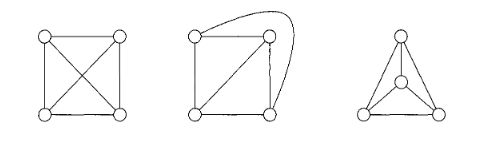
\includegraphics{images/ch1/equivalent_viz.png}
\caption{image}
\end{figure}

    \hypertarget{bipartite-graphs}{%
\subsection{2.4 Bipartite Graphs}\label{bipartite-graphs}}

Networks typically deal with relations between a single class of
entities, that is to say, the nodes are of the same type, they belong to
the same class. For example, we may be interested in citations between
cases, friendship between persons, similarity between documents and so
forth. In these examples, the entities within the classes used to
measure citations, friendship, and similarity are the same.

Yet sometimes it is interesting to consider the relationship between two
different types of elements. We might want to research, for example,
patterns of treaty ratification. Modelling this requires working with
two types of nodes: states and treaties. This implies the creation of a
bipartite network, where edges connect nodes of a different type. These
sorts of networks are sometimes also called affilation networks. Below
you can see an example of such a bipartite graph.

    \begin{tcolorbox}[breakable, size=fbox, boxrule=1pt, pad at break*=1mm,colback=cellbackground, colframe=cellborder]
\prompt{In}{incolor}{4}{\boxspacing}
\begin{Verbatim}[commandchars=\\\{\}]
\PY{n}{g\PYZus{}treaties} \PY{o}{=} \PY{n}{load\PYZus{}graph\PYZus{}from\PYZus{}json}\PY{p}{(}\PY{l+s+s2}{\PYZdq{}}\PY{l+s+s2}{data/g\PYZus{}treaties.json}\PY{l+s+s2}{\PYZdq{}}\PY{p}{)}
\PY{n}{states} \PY{o}{=} \PY{p}{[}\PY{n}{x}\PY{p}{[}\PY{l+m+mi}{0}\PY{p}{]} \PY{k}{for} \PY{n}{x} \PY{o+ow}{in} \PY{n+nb}{list}\PY{p}{(}\PY{n}{g\PYZus{}treaties}\PY{o}{.}\PY{n}{nodes}\PY{p}{(}\PY{n}{data}\PY{o}{=}\PY{l+s+s2}{\PYZdq{}}\PY{l+s+s2}{bipartite}\PY{l+s+s2}{\PYZdq{}}\PY{p}{)}\PY{p}{)} \PY{k}{if} \PY{n}{x}\PY{p}{[}\PY{l+m+mi}{1}\PY{p}{]} \PY{o}{==} \PY{l+m+mi}{0}\PY{p}{]}
\PY{n}{treaties} \PY{o}{=} \PY{p}{[}\PY{n}{x}\PY{p}{[}\PY{l+m+mi}{0}\PY{p}{]} \PY{k}{for} \PY{n}{x} \PY{o+ow}{in} \PY{n+nb}{list}\PY{p}{(}\PY{n}{g\PYZus{}treaties}\PY{o}{.}\PY{n}{nodes}\PY{p}{(}\PY{n}{data}\PY{o}{=}\PY{l+s+s2}{\PYZdq{}}\PY{l+s+s2}{bipartite}\PY{l+s+s2}{\PYZdq{}}\PY{p}{)}\PY{p}{)} \PY{k}{if} \PY{n}{x}\PY{p}{[}\PY{l+m+mi}{1}\PY{p}{]} \PY{o}{==} \PY{l+m+mi}{1}\PY{p}{]}
\PY{n}{plt}\PY{o}{.}\PY{n}{figure}\PY{p}{(}\PY{n}{figsize}\PY{o}{=}\PY{p}{(}\PY{l+m+mi}{8}\PY{p}{,}\PY{l+m+mi}{8}\PY{p}{)}\PY{p}{)}
\PY{n}{pos} \PY{o}{=} \PY{n}{nx}\PY{o}{.}\PY{n}{spring\PYZus{}layout}\PY{p}{(}\PY{n}{g\PYZus{}treaties}\PY{p}{,} \PY{n}{seed}\PY{o}{=}\PY{l+m+mi}{123}\PY{p}{)}
\PY{n}{nx}\PY{o}{.}\PY{n}{draw\PYZus{}networkx\PYZus{}nodes}\PY{p}{(}\PY{n}{g\PYZus{}treaties}\PY{p}{,} \PY{n}{pos}\PY{o}{=}\PY{n}{pos}\PY{p}{,} \PY{n}{nodelist}\PY{o}{=} \PY{n}{states}\PY{p}{,} \PY{n}{node\PYZus{}color}\PY{o}{=}\PY{l+s+s1}{\PYZsq{}}\PY{l+s+s1}{tab:blue}\PY{l+s+s1}{\PYZsq{}}\PY{p}{,} \PY{n}{alpha} \PY{o}{=} \PY{l+m+mf}{0.7}\PY{p}{)}
\PY{n}{nx}\PY{o}{.}\PY{n}{draw\PYZus{}networkx\PYZus{}nodes}\PY{p}{(}\PY{n}{g\PYZus{}treaties}\PY{p}{,} \PY{n}{pos}\PY{o}{=}\PY{n}{pos}\PY{p}{,} \PY{n}{nodelist}\PY{o}{=} \PY{n}{treaties}\PY{p}{,} \PY{n}{node\PYZus{}color}\PY{o}{=}\PY{l+s+s1}{\PYZsq{}}\PY{l+s+s1}{tab:red}\PY{l+s+s1}{\PYZsq{}}\PY{p}{,} \PY{n}{alpha} \PY{o}{=}\PY{l+m+mf}{0.7}\PY{p}{)}
\PY{n}{nx}\PY{o}{.}\PY{n}{draw\PYZus{}networkx\PYZus{}edges}\PY{p}{(}\PY{n}{g\PYZus{}treaties}\PY{p}{,} \PY{n}{pos}\PY{o}{=}\PY{n}{pos}\PY{p}{)}
\PY{n}{nx}\PY{o}{.}\PY{n}{draw\PYZus{}networkx\PYZus{}labels}\PY{p}{(}\PY{n}{g\PYZus{}treaties}\PY{p}{,} \PY{n}{pos}\PY{o}{=}\PY{n}{pos}\PY{p}{)}\PY{p}{;}
\end{Verbatim}
\end{tcolorbox}

    \begin{center}
    \adjustimage{max size={0.9\linewidth}{0.9\paperheight}}{chapters/Chapter_2_Key_Concepts/output_9_0.png}
    \end{center}
    { \hspace*{\fill} \\}
    
    The drone network that was initially created in the research was not a
bipartite network. We can, however, create one by adding information on
the types of laws to the previous network. Nodes 2019R0945, 2019R0947,
2021R0664, and 2021R0665 are drone-specific laws, meaning that they
consist of rules that specifically apply to drones. In contrast, the
other laws include rules that may be relevant to drones but are not
specifically drafted with drones in mind. Think of rules on aviation or
perhaps privacy or cybersecurity. The visualization shows which laws are
considered drone-specific legislation and which ones are not.

    \begin{tcolorbox}[breakable, size=fbox, boxrule=1pt, pad at break*=1mm,colback=cellbackground, colframe=cellborder]
\prompt{In}{incolor}{5}{\boxspacing}
\begin{Verbatim}[commandchars=\\\{\}]
\PY{c+c1}{\PYZsh{} Load the JSON data}
\PY{k}{with} \PY{n+nb}{open}\PY{p}{(}\PY{l+s+s2}{\PYZdq{}}\PY{l+s+s2}{data/drone\PYZus{}laws/g\PYZus{}dronelaws\PYZus{}1.json}\PY{l+s+s2}{\PYZdq{}}\PY{p}{)} \PY{k}{as} \PY{n}{f}\PY{p}{:}
    \PY{n}{data} \PY{o}{=} \PY{n}{json}\PY{o}{.}\PY{n}{load}\PY{p}{(}\PY{n}{f}\PY{p}{)}

\PY{c+c1}{\PYZsh{} Create a bipartite graph}
\PY{n}{B} \PY{o}{=} \PY{n}{nx}\PY{o}{.}\PY{n}{Graph}\PY{p}{(}\PY{p}{)}

\PY{c+c1}{\PYZsh{} Define drone\PYZhy{}specific and general\PYZhy{}purpose laws}
\PY{n}{drone\PYZus{}specific\PYZus{}laws} \PY{o}{=} \PY{p}{\PYZob{}}\PY{l+s+s2}{\PYZdq{}}\PY{l+s+s2}{2019R0947}\PY{l+s+s2}{\PYZdq{}}\PY{p}{,} \PY{l+s+s2}{\PYZdq{}}\PY{l+s+s2}{2021R0664}\PY{l+s+s2}{\PYZdq{}}\PY{p}{,} \PY{l+s+s2}{\PYZdq{}}\PY{l+s+s2}{2021R0665}\PY{l+s+s2}{\PYZdq{}}\PY{p}{,} \PY{l+s+s2}{\PYZdq{}}\PY{l+s+s2}{2019R0945}\PY{l+s+s2}{\PYZdq{}}\PY{p}{\PYZcb{}}
\PY{n}{general\PYZus{}purpose\PYZus{}laws} \PY{o}{=} \PY{n+nb}{set}\PY{p}{(}\PY{p}{)}

\PY{c+c1}{\PYZsh{} Add nodes for laws and categories}
\PY{k}{for} \PY{n}{node} \PY{o+ow}{in} \PY{n}{data}\PY{p}{[}\PY{l+s+s1}{\PYZsq{}}\PY{l+s+s1}{nodes}\PY{l+s+s1}{\PYZsq{}}\PY{p}{]}\PY{p}{:}
    \PY{n}{law\PYZus{}id} \PY{o}{=} \PY{n}{node}\PY{p}{[}\PY{l+s+s1}{\PYZsq{}}\PY{l+s+s1}{id}\PY{l+s+s1}{\PYZsq{}}\PY{p}{]}
    \PY{n}{B}\PY{o}{.}\PY{n}{add\PYZus{}node}\PY{p}{(}\PY{n}{law\PYZus{}id}\PY{p}{)}  \PY{c+c1}{\PYZsh{} Add law nodes}
    \PY{k}{if} \PY{n}{law\PYZus{}id} \PY{o+ow}{in} \PY{n}{drone\PYZus{}specific\PYZus{}laws}\PY{p}{:}
        \PY{n}{B}\PY{o}{.}\PY{n}{add\PYZus{}node}\PY{p}{(}\PY{l+s+s2}{\PYZdq{}}\PY{l+s+s2}{Drone Specific}\PY{l+s+s2}{\PYZdq{}}\PY{p}{)}  \PY{c+c1}{\PYZsh{} Add drone\PYZhy{}specific category node}
        \PY{n}{B}\PY{o}{.}\PY{n}{add\PYZus{}edge}\PY{p}{(}\PY{n}{law\PYZus{}id}\PY{p}{,} \PY{l+s+s2}{\PYZdq{}}\PY{l+s+s2}{Drone Specific}\PY{l+s+s2}{\PYZdq{}}\PY{p}{)}  \PY{c+c1}{\PYZsh{} Connect law to its category}
    \PY{k}{else}\PY{p}{:}
        \PY{n}{B}\PY{o}{.}\PY{n}{add\PYZus{}node}\PY{p}{(}\PY{l+s+s2}{\PYZdq{}}\PY{l+s+s2}{NOT Drone Specific}\PY{l+s+s2}{\PYZdq{}}\PY{p}{)}  \PY{c+c1}{\PYZsh{} Add general\PYZhy{}purpose category node}
        \PY{n}{B}\PY{o}{.}\PY{n}{add\PYZus{}edge}\PY{p}{(}\PY{n}{law\PYZus{}id}\PY{p}{,} \PY{l+s+s2}{\PYZdq{}}\PY{l+s+s2}{NOT Drone Specific}\PY{l+s+s2}{\PYZdq{}}\PY{p}{)}  \PY{c+c1}{\PYZsh{} Connect law to its category}
        \PY{n}{general\PYZus{}purpose\PYZus{}laws}\PY{o}{.}\PY{n}{add}\PY{p}{(}\PY{n}{law\PYZus{}id}\PY{p}{)}

\PY{c+c1}{\PYZsh{} Add edges from the original links to the bipartite graph}
\PY{k}{for} \PY{n}{link} \PY{o+ow}{in} \PY{n}{data}\PY{p}{[}\PY{l+s+s1}{\PYZsq{}}\PY{l+s+s1}{links}\PY{l+s+s1}{\PYZsq{}}\PY{p}{]}\PY{p}{:}
    \PY{n}{source} \PY{o}{=} \PY{n}{link}\PY{p}{[}\PY{l+s+s1}{\PYZsq{}}\PY{l+s+s1}{source}\PY{l+s+s1}{\PYZsq{}}\PY{p}{]}
    \PY{n}{target} \PY{o}{=} \PY{n}{link}\PY{p}{[}\PY{l+s+s1}{\PYZsq{}}\PY{l+s+s1}{target}\PY{l+s+s1}{\PYZsq{}}\PY{p}{]}
    \PY{n}{B}\PY{o}{.}\PY{n}{add\PYZus{}edge}\PY{p}{(}\PY{n}{source}\PY{p}{,} \PY{n}{target}\PY{p}{)}

\PY{c+c1}{\PYZsh{} Define colors for categories and laws}
\PY{n}{law\PYZus{}color} \PY{o}{=} \PY{l+s+s1}{\PYZsq{}}\PY{l+s+s1}{lightblue}\PY{l+s+s1}{\PYZsq{}}         \PY{c+c1}{\PYZsh{} Color for law nodes}
\PY{n}{category\PYZus{}color} \PY{o}{=} \PY{p}{\PYZob{}}\PY{l+s+s1}{\PYZsq{}}\PY{l+s+s1}{Drone Specific}\PY{l+s+s1}{\PYZsq{}}\PY{p}{:} \PY{l+s+s1}{\PYZsq{}}\PY{l+s+s1}{lightgreen}\PY{l+s+s1}{\PYZsq{}}\PY{p}{,} \PY{l+s+s1}{\PYZsq{}}\PY{l+s+s1}{NOT Drone Specific}\PY{l+s+s1}{\PYZsq{}}\PY{p}{:} \PY{l+s+s1}{\PYZsq{}}\PY{l+s+s1}{salmon}\PY{l+s+s1}{\PYZsq{}}\PY{p}{\PYZcb{}}  \PY{c+c1}{\PYZsh{} Colors for categories}

\PY{c+c1}{\PYZsh{} Create lists for node colors}
\PY{n}{node\PYZus{}colors} \PY{o}{=} \PY{p}{[}\PY{p}{]}
\PY{k}{for} \PY{n}{node} \PY{o+ow}{in} \PY{n}{B}\PY{o}{.}\PY{n}{nodes}\PY{p}{(}\PY{p}{)}\PY{p}{:}
    \PY{k}{if} \PY{n}{node} \PY{o+ow}{in} \PY{n}{category\PYZus{}color}\PY{p}{:}  \PY{c+c1}{\PYZsh{} If it\PYZsq{}s a category node}
        \PY{n}{node\PYZus{}colors}\PY{o}{.}\PY{n}{append}\PY{p}{(}\PY{n}{category\PYZus{}color}\PY{p}{[}\PY{n}{node}\PY{p}{]}\PY{p}{)}
    \PY{k}{else}\PY{p}{:}
        \PY{n}{node\PYZus{}colors}\PY{o}{.}\PY{n}{append}\PY{p}{(}\PY{n}{law\PYZus{}color}\PY{p}{)}  \PY{c+c1}{\PYZsh{} Law nodes color}

\PY{c+c1}{\PYZsh{} Visualize the bipartite graph}
\PY{n}{plt}\PY{o}{.}\PY{n}{figure}\PY{p}{(}\PY{n}{figsize}\PY{o}{=}\PY{p}{(}\PY{l+m+mi}{6}\PY{p}{,} \PY{l+m+mi}{6}\PY{p}{)}\PY{p}{)}
\PY{n}{pos} \PY{o}{=} \PY{n}{nx}\PY{o}{.}\PY{n}{spring\PYZus{}layout}\PY{p}{(}\PY{n}{B}\PY{p}{)}  \PY{c+c1}{\PYZsh{} Positions for all nodes}

\PY{c+c1}{\PYZsh{} Draw the graph with specified colors}
\PY{n}{nx}\PY{o}{.}\PY{n}{draw}\PY{p}{(}\PY{n}{B}\PY{p}{,} \PY{n}{pos}\PY{p}{,} \PY{n}{with\PYZus{}labels}\PY{o}{=}\PY{k+kc}{True}\PY{p}{,} \PY{n}{node\PYZus{}size}\PY{o}{=}\PY{l+m+mi}{700}\PY{p}{,} \PY{n}{node\PYZus{}color}\PY{o}{=}\PY{n}{node\PYZus{}colors}\PY{p}{,} \PY{n}{font\PYZus{}size}\PY{o}{=}\PY{l+m+mi}{10}\PY{p}{,} \PY{n}{font\PYZus{}weight}\PY{o}{=}\PY{l+s+s1}{\PYZsq{}}\PY{l+s+s1}{bold}\PY{l+s+s1}{\PYZsq{}}\PY{p}{,} \PY{n}{arrows}\PY{o}{=}\PY{k+kc}{False}\PY{p}{)}
\PY{n}{plt}\PY{o}{.}\PY{n}{title}\PY{p}{(}\PY{l+s+s2}{\PYZdq{}}\PY{l+s+s2}{Bipartite Network of Drone Laws}\PY{l+s+s2}{\PYZdq{}}\PY{p}{)}
\PY{n}{plt}\PY{o}{.}\PY{n}{figtext}\PY{p}{(}\PY{l+m+mf}{0.5}\PY{p}{,} \PY{l+m+mf}{0.01}\PY{p}{,} \PY{l+s+s2}{\PYZdq{}}\PY{l+s+s2}{Nodes represent laws (CELEX IDs) and categories (Drone Specific | NOT Drone Specific)}\PY{l+s+s2}{\PYZdq{}}\PY{p}{,} 
             \PY{n}{wrap}\PY{o}{=}\PY{k+kc}{True}\PY{p}{,} \PY{n}{horizontalalignment}\PY{o}{=}\PY{l+s+s1}{\PYZsq{}}\PY{l+s+s1}{center}\PY{l+s+s1}{\PYZsq{}}\PY{p}{,} \PY{n}{fontsize}\PY{o}{=}\PY{l+m+mi}{12}\PY{p}{)}
\PY{n}{plt}\PY{o}{.}\PY{n}{show}\PY{p}{(}\PY{p}{)}
\end{Verbatim}
\end{tcolorbox}

    \begin{center}
    \adjustimage{max size={0.9\linewidth}{0.9\paperheight}}{chapters/Chapter_2_Key_Concepts/output_11_0.png}
    \end{center}
    { \hspace*{\fill} \\}
    
    \hypertarget{directed-acyclic-graph-dag}{%
\subsection{2.5 Directed Acyclic Graph
(DAG)}\label{directed-acyclic-graph-dag}}

Another special type of graph is a directed acyclic graph or DAG. A DAG
is a directed graph that has no cycles or loops, hence it is `acyclic'.

Citation networks, which are often used in legal network analysis,
should in theory be DAGs. In case law citation networks, for instance,
newer cases will cite older cases and not the other way around.
Likewise, cases are unlikely to cite themselves. As a result, there
should in theory be no loops in case citation networks. In practice,
however, this does not always hold. Loops may occur, for instance if two
cases cite that both been written around the same time cite one another.
Our drone legislation example is also a DAG. It is directed, because one
law cites another, it is acyclic, because more recent legislation cites
less recent legislation and not the other way around, and it is a graph
that consists of nodes and edges.

DAGs are important in some areas of research. For example, DAGs are used
to model causal processes, on the understanding that causation is always
linear and undirectional. To illustrate, we draw a toy example of a
casual model that predicts a country will ratify a free trade treaty if
the country is democratic, has a liberal government, has high
unemployment, and a high percentage of young citizens.

Notice that, in this model, the relationship is directional and not
cyclic (once the free trade treaty is ratified, this does not, in turn,
make it more likely that democracy will prevail).

This work does not delve further into DAGs.

    \begin{tcolorbox}[breakable, size=fbox, boxrule=1pt, pad at break*=1mm,colback=cellbackground, colframe=cellborder]
\prompt{In}{incolor}{6}{\boxspacing}
\begin{Verbatim}[commandchars=\\\{\}]
\PY{n}{g\PYZus{}dag} \PY{o}{=} \PY{n}{nx}\PY{o}{.}\PY{n}{DiGraph}\PY{p}{(}\PY{p}{)}
\PY{n}{g\PYZus{}dag}\PY{o}{.}\PY{n}{add\PYZus{}edge}\PY{p}{(}\PY{l+s+s2}{\PYZdq{}}\PY{l+s+s2}{democratic}\PY{l+s+s2}{\PYZdq{}}\PY{p}{,} \PY{l+s+s2}{\PYZdq{}}\PY{l+s+s2}{liberal gov}\PY{l+s+s2}{\PYZdq{}}\PY{p}{)}
\PY{n}{g\PYZus{}dag}\PY{o}{.}\PY{n}{add\PYZus{}edge}\PY{p}{(}\PY{l+s+s2}{\PYZdq{}}\PY{l+s+s2}{liberal gov}\PY{l+s+s2}{\PYZdq{}}\PY{p}{,} \PY{l+s+s2}{\PYZdq{}}\PY{l+s+s2}{free\PYZus{}trade ratified}\PY{l+s+s2}{\PYZdq{}}\PY{p}{)}
\PY{n}{g\PYZus{}dag}\PY{o}{.}\PY{n}{add\PYZus{}edge}\PY{p}{(}\PY{l+s+s2}{\PYZdq{}}\PY{l+s+s2}{young cit}\PY{l+s+s2}{\PYZdq{}}\PY{p}{,} \PY{l+s+s2}{\PYZdq{}}\PY{l+s+s2}{free\PYZus{}trade ratified}\PY{l+s+s2}{\PYZdq{}}\PY{p}{)}
\PY{n}{g\PYZus{}dag}\PY{o}{.}\PY{n}{add\PYZus{}edge}\PY{p}{(}\PY{l+s+s2}{\PYZdq{}}\PY{l+s+s2}{high unemployment}\PY{l+s+s2}{\PYZdq{}}\PY{p}{,} \PY{l+s+s2}{\PYZdq{}}\PY{l+s+s2}{free\PYZus{}trade ratified}\PY{l+s+s2}{\PYZdq{}}\PY{p}{)}

\PY{n}{draw\PYZus{}spring}\PY{p}{(}\PY{n}{g\PYZus{}dag}\PY{p}{)}
\end{Verbatim}
\end{tcolorbox}

    \begin{center}
    \adjustimage{max size={0.9\linewidth}{0.9\paperheight}}{chapters/Chapter_2_Key_Concepts/output_13_0.png}
    \end{center}
    { \hspace*{\fill} \\}
    
    \hypertarget{trees}{%
\subsection{2.6 Trees}\label{trees}}

There are many types of trees. An intuitive one is the ``rooted tree'',
which parallels what we may naively understand as a tree: graphs without
loops with a single root node to which all the other nodes are connected
(directly or indirectly).

Trees can have a parameter controlling in how many segments they branch
out, and another controlling their height or depth, that is in this
case, how far away the furthest leaf is from the root. Here we can see a
binary tree of height 3.

    \begin{tcolorbox}[breakable, size=fbox, boxrule=1pt, pad at break*=1mm,colback=cellbackground, colframe=cellborder]
\prompt{In}{incolor}{7}{\boxspacing}
\begin{Verbatim}[commandchars=\\\{\}]
\PY{n}{g\PYZus{}tree} \PY{o}{=} \PY{n}{nx}\PY{o}{.}\PY{n}{Graph}\PY{p}{(}\PY{p}{)}
\PY{n}{g\PYZus{}tree}\PY{o}{.}\PY{n}{add\PYZus{}nodes\PYZus{}from}\PY{p}{(}\PY{p}{[}\PY{l+s+s2}{\PYZdq{}}\PY{l+s+s2}{root}\PY{l+s+s2}{\PYZdq{}}\PY{p}{,} \PY{l+m+mi}{1}\PY{p}{,} \PY{l+m+mi}{2}\PY{p}{,} \PY{l+m+mi}{3}\PY{p}{,} \PY{l+m+mi}{4}\PY{p}{,} \PY{l+m+mi}{5}\PY{p}{,} \PY{l+m+mi}{6}\PY{p}{,} \PY{l+m+mi}{7}\PY{p}{,} \PY{l+m+mi}{8}\PY{p}{,} \PY{l+m+mi}{9}\PY{p}{,} \PY{l+m+mi}{10}\PY{p}{,} \PY{l+m+mi}{11}\PY{p}{,} \PY{l+m+mi}{12}\PY{p}{,} \PY{l+m+mi}{13}\PY{p}{,} \PY{l+m+mi}{14}\PY{p}{]}\PY{p}{)}
\PY{n}{g\PYZus{}tree}\PY{o}{.}\PY{n}{add\PYZus{}edges\PYZus{}from}\PY{p}{(}\PY{p}{[}\PY{p}{(}\PY{l+s+s2}{\PYZdq{}}\PY{l+s+s2}{root}\PY{l+s+s2}{\PYZdq{}}\PY{p}{,}\PY{l+m+mi}{1}\PY{p}{)}\PY{p}{,}\PY{p}{(}\PY{l+s+s2}{\PYZdq{}}\PY{l+s+s2}{root}\PY{l+s+s2}{\PYZdq{}}\PY{p}{,}\PY{l+m+mi}{2}\PY{p}{)}\PY{p}{,}\PY{p}{(}\PY{l+m+mi}{1}\PY{p}{,}\PY{l+m+mi}{3}\PY{p}{)}\PY{p}{,}\PY{p}{(}\PY{l+m+mi}{1}\PY{p}{,}\PY{l+m+mi}{4}\PY{p}{)}\PY{p}{,}\PY{p}{(}\PY{l+m+mi}{2}\PY{p}{,}\PY{l+m+mi}{5}\PY{p}{)}\PY{p}{,}\PY{p}{(}\PY{l+m+mi}{2}\PY{p}{,}\PY{l+m+mi}{6}\PY{p}{)}\PY{p}{,}\PY{p}{(}\PY{l+m+mi}{3}\PY{p}{,}\PY{l+m+mi}{7}\PY{p}{)}\PY{p}{,}\PY{p}{(}\PY{l+m+mi}{3}\PY{p}{,}\PY{l+m+mi}{8}\PY{p}{)}\PY{p}{,}
                       \PY{p}{(}\PY{l+m+mi}{4}\PY{p}{,}\PY{l+m+mi}{9}\PY{p}{)}\PY{p}{,}\PY{p}{(}\PY{l+m+mi}{4}\PY{p}{,}\PY{l+m+mi}{10}\PY{p}{)}\PY{p}{,}\PY{p}{(}\PY{l+m+mi}{5}\PY{p}{,}\PY{l+m+mi}{11}\PY{p}{)}\PY{p}{,}\PY{p}{(}\PY{l+m+mi}{5}\PY{p}{,}\PY{l+m+mi}{12}\PY{p}{)}\PY{p}{,}\PY{p}{(}\PY{l+m+mi}{6}\PY{p}{,}\PY{l+m+mi}{13}\PY{p}{)}\PY{p}{,}\PY{p}{(}\PY{l+m+mi}{6}\PY{p}{,}\PY{l+m+mi}{14}\PY{p}{)}\PY{p}{]}\PY{p}{)}
\PY{n}{draw\PYZus{}spring}\PY{p}{(}\PY{n}{g\PYZus{}tree}\PY{p}{)}
\end{Verbatim}
\end{tcolorbox}

    \begin{center}
    \adjustimage{max size={0.9\linewidth}{0.9\paperheight}}{chapters/Chapter_2_Key_Concepts/output_15_0.png}
    \end{center}
    { \hspace*{\fill} \\}
    
    Trees can be directed or undirected. Directed trees can flow from the
root out towards the leaves, or vice versa, flow from the leaves into
the root. Trees are not necessarily rooted.

There is a great variety of trees, and the tree data structure is widely
used by many disciplines. This work does not delve further into trees.

    \hypertarget{graphs-versus-networks}{%
\subsection{2.7 Graphs versus Networks}\label{graphs-versus-networks}}

Graphs and networks are sometimes used interchangeably. However, the
terms point to different aspects of the graph structure and to different
fields of study.

At the graph level, it is irrelevant wether the nodes and edges
represent friendship relations, connections between subway stations, or
participation in a criminal organization. The focus is on the nodes and
edges are considered abstractly. Graph theory is a field of mathematics
that explores the abstract properties of graphs.

Networks are based on graphs (hence on nodes and edges), but they are
used to study concrete relationships between entities: treaty
ratifications by states, citations between court cases, similarity
between documents, etc. Moreover, the nodes and edges can be enriched
with even more information (which may be called metadata, see Chapter 2,
sections 5 and 6). For example, if nodes consist of documents, a network
might record the language of the documents, the name of the authors, the
year of publication, etc.

    \hypertarget{power-law-distribution}{%
\subsection{2.8 Power Law Distribution}\label{power-law-distribution}}

Networks frequently have a Power Law distribution. A Power Law
distribution entails that the frequency distributions of network
properties are highly skewed. For example, it is common in legal network
analysis, particularly the analysis of citation networks, that a few
nodes have a very high number of edges and most nodes a small number of
edges. We illustrate this by means of a network of Court of Justice of
the European Union (CJEU) case law, where the source nodes consist of
cases that are labeled as `consumer protection'. With source nodes, we
mean the cases that were searched and for which the citations in those
cases were harvested. In this network, the cases are the nodes and the
references in and to the cases the edges. The network consists of 1,614
nodes (cases) and 2,662 edges (references).

Below, we plot the distribution of incoming citations among the cases by
means of a histogram. The horizontal axis shows the number of incoming
citations and the vertical axis the number of cases. The results reveal
that a relatively small number of cases have a relatively high number of
incoming citations (the sparse right tail of the histogram recording 40
or more citations), whereas there are a lot of cases that are hardly
ever, if at all, cited (the towering bar recording cases with around 0
citations).

    \begin{tcolorbox}[breakable, size=fbox, boxrule=1pt, pad at break*=1mm,colback=cellbackground, colframe=cellborder]
\prompt{In}{incolor}{8}{\boxspacing}
\begin{Verbatim}[commandchars=\\\{\}]
\PY{n}{g\PYZus{}consprot} \PY{o}{=} \PY{n}{load\PYZus{}graph\PYZus{}from\PYZus{}json}\PY{p}{(}\PY{l+s+s2}{\PYZdq{}}\PY{l+s+s2}{data/g\PYZus{}consprot.json}\PY{l+s+s2}{\PYZdq{}}\PY{p}{)}
\PY{n}{plt}\PY{o}{.}\PY{n}{figure}\PY{p}{(}\PY{n}{figsize}\PY{o}{=}\PY{p}{(}\PY{l+m+mi}{4}\PY{p}{,}\PY{l+m+mi}{4}\PY{p}{)}\PY{p}{)}
\PY{n}{plt}\PY{o}{.}\PY{n}{title}\PY{p}{(}\PY{l+s+s2}{\PYZdq{}}\PY{l+s+s2}{Power Law Distribution Consumer Protection Case Law Citation Network}\PY{l+s+s2}{\PYZdq{}}\PY{p}{)}
\PY{n}{plt}\PY{o}{.}\PY{n}{xlabel}\PY{p}{(}\PY{l+s+s2}{\PYZdq{}}\PY{l+s+s2}{\PYZsh{} of Incoming Citations}\PY{l+s+s2}{\PYZdq{}}\PY{p}{)} \PY{c+c1}{\PYZsh{}add label}
\PY{n}{plt}\PY{o}{.}\PY{n}{ylabel}\PY{p}{(}\PY{l+s+s2}{\PYZdq{}}\PY{l+s+s2}{\PYZsh{} of Court Decisions}\PY{l+s+s2}{\PYZdq{}}\PY{p}{)} \PY{c+c1}{\PYZsh{}add label}
\PY{n}{sns}\PY{o}{.}\PY{n}{histplot}\PY{p}{(}\PY{n+nb}{dict}\PY{p}{(}\PY{n}{g\PYZus{}consprot}\PY{o}{.}\PY{n}{in\PYZus{}degree}\PY{p}{)}\PY{o}{.}\PY{n}{values}\PY{p}{(}\PY{p}{)}\PY{p}{,} \PY{n}{stat}\PY{o}{=}\PY{l+s+s2}{\PYZdq{}}\PY{l+s+s2}{count}\PY{l+s+s2}{\PYZdq{}}\PY{p}{,} \PY{n}{bins}\PY{o}{=}\PY{l+m+mi}{20}\PY{p}{,} \PY{n}{kde}\PY{o}{=}\PY{k+kc}{True}\PY{p}{)}\PY{p}{;} 
\end{Verbatim}
\end{tcolorbox}

    \begin{center}
    \adjustimage{max size={0.9\linewidth}{0.9\paperheight}}{chapters/Chapter_2_Key_Concepts/output_19_0.png}
    \end{center}
    { \hspace*{\fill} \\}
    
    We can also observe a power law distribution in our drone legislation
example. Cleary, the vast majority of laws hardly have citations,
whereas a small number of laws have a substantial number of citations.

    \begin{tcolorbox}[breakable, size=fbox, boxrule=1pt, pad at break*=1mm,colback=cellbackground, colframe=cellborder]
\prompt{In}{incolor}{9}{\boxspacing}
\begin{Verbatim}[commandchars=\\\{\}]
\PY{n}{plt}\PY{o}{.}\PY{n}{figure}\PY{p}{(}\PY{n}{figsize}\PY{o}{=}\PY{p}{(}\PY{l+m+mi}{4}\PY{p}{,}\PY{l+m+mi}{4}\PY{p}{)}\PY{p}{)}
\PY{n}{plt}\PY{o}{.}\PY{n}{title}\PY{p}{(}\PY{l+s+s2}{\PYZdq{}}\PY{l+s+s2}{Power Law Distribution Drone Legislation Network}\PY{l+s+s2}{\PYZdq{}}\PY{p}{)}
\PY{n}{plt}\PY{o}{.}\PY{n}{xlabel}\PY{p}{(}\PY{l+s+s2}{\PYZdq{}}\PY{l+s+s2}{\PYZsh{} of Incoming+Outgoing Citations}\PY{l+s+s2}{\PYZdq{}}\PY{p}{)} \PY{c+c1}{\PYZsh{}add label}
\PY{n}{plt}\PY{o}{.}\PY{n}{ylabel}\PY{p}{(}\PY{l+s+s2}{\PYZdq{}}\PY{l+s+s2}{\PYZsh{} of Laws}\PY{l+s+s2}{\PYZdq{}}\PY{p}{)} \PY{c+c1}{\PYZsh{}add label}
\PY{n}{sns}\PY{o}{.}\PY{n}{histplot}\PY{p}{(}\PY{n+nb}{dict}\PY{p}{(}\PY{n}{g\PYZus{}drones1}\PY{o}{.}\PY{n}{degree}\PY{p}{)}\PY{o}{.}\PY{n}{values}\PY{p}{(}\PY{p}{)}\PY{p}{,} \PY{n}{stat}\PY{o}{=}\PY{l+s+s2}{\PYZdq{}}\PY{l+s+s2}{count}\PY{l+s+s2}{\PYZdq{}}\PY{p}{,} \PY{n}{bins}\PY{o}{=}\PY{l+m+mi}{20}\PY{p}{,} \PY{n}{kde}\PY{o}{=}\PY{k+kc}{True}\PY{p}{)}\PY{p}{;} 
\end{Verbatim}
\end{tcolorbox}

    \begin{center}
    \adjustimage{max size={0.9\linewidth}{0.9\paperheight}}{chapters/Chapter_2_Key_Concepts/output_21_0.png}
    \end{center}
    { \hspace*{\fill} \\}
    
    \begin{quote}
Here we show both incoming and outgoing citations while in the consumer
protection network we focused on incoming citations. The reason for this
difference is that the drone legislation network has many laws that are
cited at least once, but very few that are not cited at all. This
happens because of how we built the network. We started with one law and
then tracked all the references made to and from that law. As a result,
the network includes many laws that have been cited at least once.
\end{quote}

    `Law' in power law distributions refers to something akin to a `law of
nature'. It does not have anything to do with the law as in norms or
rules. Rather, a power law distribution is an empirical fact of certain
networks such as citation networks or social networks.

Power Law distributions often have the effect of preferential
attachment: Ihe nodes with many edges are likely to receive more edges
(e.g., citations) in the future for the mere fact that they already had
many edges before. This is also called the `rich get richer' effect.

    \hypertarget{node-degree-and-node-centrality}{%
\subsection{2.9 Node Degree and Node
Centrality}\label{node-degree-and-node-centrality}}

Network analysis is a method to capture how central a node is in a
network. This centrality can be an indicator of, for instance, the
popularity or relevance of a node in a network.

We will discuss different metrics such as Degree Centrality, Closeness
Centrality and Betweeness Centrality in more detail in Chatper 3 of this
manual. For now, it key to note that there may be more than one way of
being `central'. Intuitively compare nodes 3, 5 and 7 in the Krackhard
kite graph below. Which one is the most important?

    \begin{tcolorbox}[breakable, size=fbox, boxrule=1pt, pad at break*=1mm,colback=cellbackground, colframe=cellborder]
\prompt{In}{incolor}{11}{\boxspacing}
\begin{Verbatim}[commandchars=\\\{\}]
\PY{n}{g\PYZus{}kite} \PY{o}{=} \PY{n}{nx}\PY{o}{.}\PY{n}{krackhardt\PYZus{}kite\PYZus{}graph}\PY{p}{(}\PY{p}{)}

\PY{n}{plt}\PY{o}{.}\PY{n}{figure}\PY{p}{(}\PY{n}{figsize}\PY{o}{=}\PY{p}{(}\PY{l+m+mi}{4}\PY{p}{,} \PY{l+m+mi}{2}\PY{p}{)}\PY{p}{)}  
\PY{n}{pos} \PY{o}{=} \PY{n}{nx}\PY{o}{.}\PY{n}{spring\PYZus{}layout}\PY{p}{(}\PY{n}{g\PYZus{}kite}\PY{p}{,} \PY{n}{seed}\PY{o}{=}\PY{l+m+mi}{10}\PY{p}{)}  \PY{c+c1}{\PYZsh{} Fixed layout with a seed}
\PY{n}{nx}\PY{o}{.}\PY{n}{draw}\PY{p}{(}\PY{n}{g\PYZus{}kite}\PY{p}{,} \PY{n}{pos}\PY{p}{,} \PY{n}{with\PYZus{}labels}\PY{o}{=}\PY{k+kc}{True}\PY{p}{)} 
\PY{n}{plt}\PY{o}{.}\PY{n}{show}\PY{p}{(}\PY{p}{)}
\end{Verbatim}
\end{tcolorbox}

    \begin{center}
    \adjustimage{max size={0.9\linewidth}{0.9\paperheight}}{chapters/Chapter_2_Key_Concepts/output_25_0.png}
    \end{center}
    { \hspace*{\fill} \\}
    
    The answer to this question depends on how `importance' is
operationalized. If we define importance as the node with the most
connections, node 3 (six edges) and perhaps nodes 5 and 6 (five edges
each) come to mind. However, node 3 is rather far removed from other
nodes in the network, such as nodes 8 and 9. It takes three steps to
reach node 8 and four steps to reach node 9 from node 3. From this
perspective, nodes 5 and 6 might be considered more important, as we can
reach most nodes in one step, some in two, and one in three steps.
Another way to look at importance is to focus on the nodes that `glue'
the network together. In the kite graph, removing node 7 would result in
nodes 8 and 9 being disconnected from the rest of the network. To a
lesser extent, node 8 also causes a disconnect.

    We can do a similar exercise for our drone network. Here we can observe
that node 2019R0945 is the most connected node in terms of `glue',
number of direct neighbors, and shortest paths to other nodes in the
network. Node 2021R0664 is also well-connected, but to a much lesser
extent than node 2019R0945.

    \begin{tcolorbox}[breakable, size=fbox, boxrule=1pt, pad at break*=1mm,colback=cellbackground, colframe=cellborder]
\prompt{In}{incolor}{13}{\boxspacing}
\begin{Verbatim}[commandchars=\\\{\}]
\PY{c+c1}{\PYZsh{} Visualize the graph}
\PY{n}{plt}\PY{o}{.}\PY{n}{figure}\PY{p}{(}\PY{n}{figsize}\PY{o}{=}\PY{p}{(}\PY{l+m+mi}{6}\PY{p}{,} \PY{l+m+mi}{6}\PY{p}{)}\PY{p}{)}
\PY{n}{pos} \PY{o}{=} \PY{n}{nx}\PY{o}{.}\PY{n}{spring\PYZus{}layout}\PY{p}{(}\PY{n}{g\PYZus{}drones1}\PY{p}{)} 
\PY{n}{nx}\PY{o}{.}\PY{n}{draw}\PY{p}{(}\PY{n}{g\PYZus{}drones1}\PY{p}{,} \PY{n}{pos}\PY{p}{,} \PY{n}{with\PYZus{}labels}\PY{o}{=}\PY{k+kc}{True}\PY{p}{,} \PY{n}{node\PYZus{}size}\PY{o}{=}\PY{l+m+mi}{700}\PY{p}{,} \PY{n}{node\PYZus{}color}\PY{o}{=}\PY{l+s+s1}{\PYZsq{}}\PY{l+s+s1}{lightblue}\PY{l+s+s1}{\PYZsq{}}\PY{p}{,} \PY{n}{font\PYZus{}size}\PY{o}{=}\PY{l+m+mi}{10}\PY{p}{,} \PY{n}{font\PYZus{}weight}\PY{o}{=}\PY{l+s+s1}{\PYZsq{}}\PY{l+s+s1}{bold}\PY{l+s+s1}{\PYZsq{}}\PY{p}{,} \PY{n}{arrows}\PY{o}{=}\PY{k+kc}{True}\PY{p}{)}
\PY{n}{plt}\PY{o}{.}\PY{n}{title}\PY{p}{(}\PY{l+s+s2}{\PYZdq{}}\PY{l+s+s2}{Directed Graph of Drone Laws}\PY{l+s+s2}{\PYZdq{}}\PY{p}{)}
\PY{n}{plt}\PY{o}{.}\PY{n}{figtext}\PY{p}{(}\PY{l+m+mf}{0.5}\PY{p}{,} \PY{l+m+mf}{0.01}\PY{p}{,} \PY{l+s+s2}{\PYZdq{}}\PY{l+s+s2}{Node labels are CELEX IDs: Year \PYZhy{} Regulation(R)/Directive(D) \PYZhy{} Number}\PY{l+s+s2}{\PYZdq{}}\PY{p}{,} 
             \PY{n}{wrap}\PY{o}{=}\PY{k+kc}{True}\PY{p}{,} \PY{n}{horizontalalignment}\PY{o}{=}\PY{l+s+s1}{\PYZsq{}}\PY{l+s+s1}{center}\PY{l+s+s1}{\PYZsq{}}\PY{p}{,} \PY{n}{fontsize}\PY{o}{=}\PY{l+m+mi}{10}\PY{p}{)}
\PY{n}{plt}\PY{o}{.}\PY{n}{show}\PY{p}{(}\PY{p}{)}
\end{Verbatim}
\end{tcolorbox}

    \begin{center}
    \adjustimage{max size={0.9\linewidth}{0.9\paperheight}}{chapters/Chapter_2_Key_Concepts/output_28_0.png}
    \end{center}
    { \hspace*{\fill} \\}
    
    \begin{quote}
Selecting node 2019R0945 as a starting point for the network
construction makes it likely a central node in the resulting network.
This will become more clear when explain the concept of ego networks
below.
\end{quote}

    There are many different ways to look at importance (in network analysis
terminology: centrality). We will return to this in subsequent chapters.

    \hypertarget{community-detection}{%
\subsection{2.10 Community Detection}\label{community-detection}}

Network analysis allows for the detection of communities in networks,
which are sometimes also called `cliques' or `clusters'.

The idea behind community detection is to group together nodes that are
tightly connected to each other. In most scenarios, that means that the
level of connection within the nodes of a particular community will be
higher than outside of it.

Nodes that belong to the same community are likely to share common
attributes or functions, and they often possess different properties
than the larger network.

Various algorithms exist to detect communities. The Girvan-Newman
Algorithm, Label Propagation Communities and Louvain Communities will be
explored in Chapter 4. Nevertheless, we can already provide an idea of
what the clustering looks like. The plot shows two clusters, one around
2019R945, the other one around other drone-specific legislation (e.g.,
2019R947, 2021R664, 2021R665) and laws related to that legislation.

    \begin{tcolorbox}[breakable, size=fbox, boxrule=1pt, pad at break*=1mm,colback=cellbackground, colframe=cellborder]
\prompt{In}{incolor}{22}{\boxspacing}
\begin{Verbatim}[commandchars=\\\{\}]
\PY{c+c1}{\PYZsh{} Load the JSON data}
\PY{k}{with} \PY{n+nb}{open}\PY{p}{(}\PY{l+s+s2}{\PYZdq{}}\PY{l+s+s2}{data/drone\PYZus{}laws/g\PYZus{}dronelaws\PYZus{}1.json}\PY{l+s+s2}{\PYZdq{}}\PY{p}{)} \PY{k}{as} \PY{n}{f}\PY{p}{:}
    \PY{n}{data} \PY{o}{=} \PY{n}{json}\PY{o}{.}\PY{n}{load}\PY{p}{(}\PY{n}{f}\PY{p}{)}
\PY{c+c1}{\PYZsh{} Create a directed graph from the data}
\PY{n}{g\PYZus{}dag} \PY{o}{=} \PY{n}{nx}\PY{o}{.}\PY{n}{DiGraph}\PY{p}{(}\PY{p}{)}
\PY{c+c1}{\PYZsh{} Add nodes}
\PY{k}{for} \PY{n}{node} \PY{o+ow}{in} \PY{n}{data}\PY{p}{[}\PY{l+s+s1}{\PYZsq{}}\PY{l+s+s1}{nodes}\PY{l+s+s1}{\PYZsq{}}\PY{p}{]}\PY{p}{:}
    \PY{n}{g\PYZus{}dag}\PY{o}{.}\PY{n}{add\PYZus{}node}\PY{p}{(}\PY{n}{node}\PY{p}{[}\PY{l+s+s1}{\PYZsq{}}\PY{l+s+s1}{id}\PY{l+s+s1}{\PYZsq{}}\PY{p}{]}\PY{p}{)}
\PY{c+c1}{\PYZsh{} Add edges}
\PY{k}{for} \PY{n}{link} \PY{o+ow}{in} \PY{n}{data}\PY{p}{[}\PY{l+s+s1}{\PYZsq{}}\PY{l+s+s1}{links}\PY{l+s+s1}{\PYZsq{}}\PY{p}{]}\PY{p}{:}
    \PY{n}{g\PYZus{}dag}\PY{o}{.}\PY{n}{add\PYZus{}edge}\PY{p}{(}\PY{n}{link}\PY{p}{[}\PY{l+s+s1}{\PYZsq{}}\PY{l+s+s1}{source}\PY{l+s+s1}{\PYZsq{}}\PY{p}{]}\PY{p}{,} \PY{n}{link}\PY{p}{[}\PY{l+s+s1}{\PYZsq{}}\PY{l+s+s1}{target}\PY{l+s+s1}{\PYZsq{}}\PY{p}{]}\PY{p}{)}
\PY{c+c1}{\PYZsh{} Convert to undirected graph for community detection}
\PY{n}{g\PYZus{}undirected} \PY{o}{=} \PY{n}{g\PYZus{}dag}\PY{o}{.}\PY{n}{to\PYZus{}undirected}\PY{p}{(}\PY{p}{)}
\PY{c+c1}{\PYZsh{} Detect communities using the greedy modularity method}
\PY{n}{communities} \PY{o}{=} \PY{n}{community}\PY{o}{.}\PY{n}{greedy\PYZus{}modularity\PYZus{}communities}\PY{p}{(}\PY{n}{g\PYZus{}undirected}\PY{p}{)}
\PY{c+c1}{\PYZsh{} Create a color map for the communities}
\PY{n}{color\PYZus{}map} \PY{o}{=} \PY{p}{\PYZob{}}\PY{p}{\PYZcb{}}
\PY{k}{for} \PY{n}{i}\PY{p}{,} \PY{n}{comm} \PY{o+ow}{in} \PY{n+nb}{enumerate}\PY{p}{(}\PY{n}{communities}\PY{p}{)}\PY{p}{:}
    \PY{k}{for} \PY{n}{node} \PY{o+ow}{in} \PY{n}{comm}\PY{p}{:}
        \PY{n}{color\PYZus{}map}\PY{p}{[}\PY{n}{node}\PY{p}{]} \PY{o}{=} \PY{n}{i}
\PY{c+c1}{\PYZsh{} Draw the graph}
\PY{n}{plt}\PY{o}{.}\PY{n}{figure}\PY{p}{(}\PY{n}{figsize}\PY{o}{=}\PY{p}{(}\PY{l+m+mi}{5}\PY{p}{,} \PY{l+m+mi}{5}\PY{p}{)}\PY{p}{)}
\PY{n}{pos} \PY{o}{=} \PY{n}{nx}\PY{o}{.}\PY{n}{spring\PYZus{}layout}\PY{p}{(}\PY{n}{g\PYZus{}undirected}\PY{p}{)}  \PY{c+c1}{\PYZsh{} positions for all nodes}
\PY{c+c1}{\PYZsh{} Draw nodes with colors based on their community}
\PY{n}{node\PYZus{}colors} \PY{o}{=} \PY{p}{[}\PY{n}{color\PYZus{}map}\PY{p}{[}\PY{n}{node}\PY{p}{]} \PY{k}{for} \PY{n}{node} \PY{o+ow}{in} \PY{n}{g\PYZus{}undirected}\PY{o}{.}\PY{n}{nodes}\PY{p}{(}\PY{p}{)}\PY{p}{]}
\PY{n}{nx}\PY{o}{.}\PY{n}{draw}\PY{p}{(}\PY{n}{g\PYZus{}undirected}\PY{p}{,} \PY{n}{pos}\PY{p}{,} \PY{n}{with\PYZus{}labels}\PY{o}{=}\PY{k+kc}{True}\PY{p}{,} \PY{n}{node\PYZus{}color}\PY{o}{=}\PY{n}{node\PYZus{}colors}\PY{p}{,} 
        \PY{n}{node\PYZus{}size}\PY{o}{=}\PY{l+m+mi}{100}\PY{p}{,} \PY{n}{font\PYZus{}size}\PY{o}{=}\PY{l+m+mi}{10}\PY{p}{,} \PY{n}{cmap}\PY{o}{=}\PY{n}{plt}\PY{o}{.}\PY{n}{cm}\PY{o}{.}\PY{n}{jet}\PY{p}{)}
\PY{c+c1}{\PYZsh{} Show the plot}
\PY{n}{plt}\PY{o}{.}\PY{n}{title}\PY{p}{(}\PY{l+s+s2}{\PYZdq{}}\PY{l+s+s2}{Drone Laws Communities}\PY{l+s+s2}{\PYZdq{}}\PY{p}{)}
\PY{n}{plt}\PY{o}{.}\PY{n}{show}\PY{p}{(}\PY{p}{)}
\end{Verbatim}
\end{tcolorbox}

    \begin{center}
    \adjustimage{max size={0.9\linewidth}{0.9\paperheight}}{chapters/Chapter_2_Key_Concepts/output_32_0.png}
    \end{center}
    { \hspace*{\fill} \\}
    
    It may be argued it is not necessary to detect communities in such a
relatively small network. We therefore expand the network. In the
network above, we included references in source node 2019R0945,
references to the source node, and references to the references to the
source node. In our new network, we select two source nodes with
drone-specific legislation (2019R0945 and 2021R0664). Furthermore, we
include in the network references in the two source nodes, the
references in the references that are in the source node, and the
references \emph{to} one of the two source nodes. The network we obtain
includes many more nodes. A closer inspection would reveal clusters of
legislation that deal with a variety of topics, ranging from clusters
with drone-specific legislation to clusters with avation-specific laws
to a cluster with privacy legislation.

    \begin{tcolorbox}[breakable, size=fbox, boxrule=1pt, pad at break*=1mm,colback=cellbackground, colframe=cellborder]
\prompt{In}{incolor}{23}{\boxspacing}
\begin{Verbatim}[commandchars=\\\{\}]
\PY{c+c1}{\PYZsh{} Load the JSON data}
\PY{k}{with} \PY{n+nb}{open}\PY{p}{(}\PY{l+s+s2}{\PYZdq{}}\PY{l+s+s2}{data/drone\PYZus{}laws/g\PYZus{}dronelaws\PYZus{}2.json}\PY{l+s+s2}{\PYZdq{}}\PY{p}{)} \PY{k}{as} \PY{n}{f}\PY{p}{:}
    \PY{n}{data} \PY{o}{=} \PY{n}{json}\PY{o}{.}\PY{n}{load}\PY{p}{(}\PY{n}{f}\PY{p}{)}
\PY{c+c1}{\PYZsh{} Create a directed graph from the data}
\PY{n}{g\PYZus{}dag} \PY{o}{=} \PY{n}{nx}\PY{o}{.}\PY{n}{DiGraph}\PY{p}{(}\PY{p}{)}
\PY{c+c1}{\PYZsh{} Add nodes}
\PY{k}{for} \PY{n}{node} \PY{o+ow}{in} \PY{n}{data}\PY{p}{[}\PY{l+s+s1}{\PYZsq{}}\PY{l+s+s1}{nodes}\PY{l+s+s1}{\PYZsq{}}\PY{p}{]}\PY{p}{:}
    \PY{n}{g\PYZus{}dag}\PY{o}{.}\PY{n}{add\PYZus{}node}\PY{p}{(}\PY{n}{node}\PY{p}{[}\PY{l+s+s1}{\PYZsq{}}\PY{l+s+s1}{id}\PY{l+s+s1}{\PYZsq{}}\PY{p}{]}\PY{p}{)}
\PY{c+c1}{\PYZsh{} Add edges}
\PY{k}{for} \PY{n}{link} \PY{o+ow}{in} \PY{n}{data}\PY{p}{[}\PY{l+s+s1}{\PYZsq{}}\PY{l+s+s1}{links}\PY{l+s+s1}{\PYZsq{}}\PY{p}{]}\PY{p}{:}
    \PY{n}{g\PYZus{}dag}\PY{o}{.}\PY{n}{add\PYZus{}edge}\PY{p}{(}\PY{n}{link}\PY{p}{[}\PY{l+s+s1}{\PYZsq{}}\PY{l+s+s1}{source}\PY{l+s+s1}{\PYZsq{}}\PY{p}{]}\PY{p}{,} \PY{n}{link}\PY{p}{[}\PY{l+s+s1}{\PYZsq{}}\PY{l+s+s1}{target}\PY{l+s+s1}{\PYZsq{}}\PY{p}{]}\PY{p}{)}
\PY{c+c1}{\PYZsh{} Convert to undirected graph for community detection}
\PY{n}{g\PYZus{}undirected} \PY{o}{=} \PY{n}{g\PYZus{}dag}\PY{o}{.}\PY{n}{to\PYZus{}undirected}\PY{p}{(}\PY{p}{)}
\PY{c+c1}{\PYZsh{} Detect communities using the greedy modularity method}
\PY{n}{communities} \PY{o}{=} \PY{n}{community}\PY{o}{.}\PY{n}{greedy\PYZus{}modularity\PYZus{}communities}\PY{p}{(}\PY{n}{g\PYZus{}undirected}\PY{p}{)}
\PY{c+c1}{\PYZsh{} Create a color map for the communities}
\PY{n}{color\PYZus{}map} \PY{o}{=} \PY{p}{\PYZob{}}\PY{p}{\PYZcb{}}
\PY{k}{for} \PY{n}{i}\PY{p}{,} \PY{n}{comm} \PY{o+ow}{in} \PY{n+nb}{enumerate}\PY{p}{(}\PY{n}{communities}\PY{p}{)}\PY{p}{:}
    \PY{k}{for} \PY{n}{node} \PY{o+ow}{in} \PY{n}{comm}\PY{p}{:}
        \PY{n}{color\PYZus{}map}\PY{p}{[}\PY{n}{node}\PY{p}{]} \PY{o}{=} \PY{n}{i}
\PY{c+c1}{\PYZsh{} Draw the graph}
\PY{n}{plt}\PY{o}{.}\PY{n}{figure}\PY{p}{(}\PY{n}{figsize}\PY{o}{=}\PY{p}{(}\PY{l+m+mi}{10}\PY{p}{,} \PY{l+m+mi}{6}\PY{p}{)}\PY{p}{)}
\PY{n}{pos} \PY{o}{=} \PY{n}{nx}\PY{o}{.}\PY{n}{spring\PYZus{}layout}\PY{p}{(}\PY{n}{g\PYZus{}undirected}\PY{p}{)}  \PY{c+c1}{\PYZsh{} positions for all nodes}
\PY{c+c1}{\PYZsh{} Draw nodes with colors based on their community}
\PY{n}{node\PYZus{}colors} \PY{o}{=} \PY{p}{[}\PY{n}{color\PYZus{}map}\PY{p}{[}\PY{n}{node}\PY{p}{]} \PY{k}{for} \PY{n}{node} \PY{o+ow}{in} \PY{n}{g\PYZus{}undirected}\PY{o}{.}\PY{n}{nodes}\PY{p}{(}\PY{p}{)}\PY{p}{]}
\PY{n}{nx}\PY{o}{.}\PY{n}{draw}\PY{p}{(}\PY{n}{g\PYZus{}undirected}\PY{p}{,} \PY{n}{pos}\PY{p}{,} \PY{n}{with\PYZus{}labels}\PY{o}{=}\PY{k+kc}{True}\PY{p}{,} \PY{n}{node\PYZus{}color}\PY{o}{=}\PY{n}{node\PYZus{}colors}\PY{p}{,} 
        \PY{n}{node\PYZus{}size}\PY{o}{=}\PY{l+m+mi}{50}\PY{p}{,} \PY{n}{font\PYZus{}size}\PY{o}{=}\PY{l+m+mi}{10}\PY{p}{,} \PY{n}{cmap}\PY{o}{=}\PY{n}{plt}\PY{o}{.}\PY{n}{cm}\PY{o}{.}\PY{n}{jet}\PY{p}{)}
\PY{c+c1}{\PYZsh{} Show the plot}
\PY{n}{plt}\PY{o}{.}\PY{n}{title}\PY{p}{(}\PY{l+s+s2}{\PYZdq{}}\PY{l+s+s2}{Drone Laws Communities}\PY{l+s+s2}{\PYZdq{}}\PY{p}{)}
\PY{n}{plt}\PY{o}{.}\PY{n}{show}\PY{p}{(}\PY{p}{)}
\end{Verbatim}
\end{tcolorbox}

    \begin{center}
    \adjustimage{max size={0.9\linewidth}{0.9\paperheight}}{chapters/Chapter_2_Key_Concepts/output_34_0.png}
    \end{center}
    { \hspace*{\fill} \\}
    
    \hypertarget{paths-shortest-paths-and-distance-between-nodes}{%
\subsection{2.11 Paths, Shortest Paths, and Distance between
Nodes}\label{paths-shortest-paths-and-distance-between-nodes}}

A path is a series of steps getting from node A to node B. For any node
of the network, it is possible to calculate the path it has to other
nodes (if such a path exists) and its distance. The distance is the
number of steps, or the number of steps weighted by any relevant weight
metric.

Some complications deserve mention here, which are further discussed
below:

\begin{itemize}
\tightlist
\item
  Disconnected nodes
\item
  Fully connected networks
\item
  Shortest path
\item
  Weighted paths
\item
  Random paths
\item
  Eccentricity and network diameter
\end{itemize}

    \hypertarget{disconnected-nodes}{%
\subsubsection{Disconnected Nodes}\label{disconnected-nodes}}

It is not guaranteed that there will be a path between two nodes. It is
possible that two sets of nodes are simply not connected. In this case
there is no path between the nodes, directly or indirectly. This
situation can be observed in the example below, where nodes A, B, and C,
are disconnected from nodes D and E.

    \begin{tcolorbox}[breakable, size=fbox, boxrule=1pt, pad at break*=1mm,colback=cellbackground, colframe=cellborder]
\prompt{In}{incolor}{24}{\boxspacing}
\begin{Verbatim}[commandchars=\\\{\}]
\PY{n}{g\PYZus{}disconnected} \PY{o}{=} \PY{n}{nx}\PY{o}{.}\PY{n}{Graph}\PY{p}{(}\PY{p}{)}
\PY{n}{g\PYZus{}disconnected}\PY{o}{.}\PY{n}{add\PYZus{}nodes\PYZus{}from}\PY{p}{(}\PY{p}{[}\PY{l+s+s1}{\PYZsq{}}\PY{l+s+s1}{A}\PY{l+s+s1}{\PYZsq{}}\PY{p}{,}\PY{l+s+s1}{\PYZsq{}}\PY{l+s+s1}{B}\PY{l+s+s1}{\PYZsq{}}\PY{p}{,}\PY{l+s+s1}{\PYZsq{}}\PY{l+s+s1}{C}\PY{l+s+s1}{\PYZsq{}}\PY{p}{,}\PY{l+s+s1}{\PYZsq{}}\PY{l+s+s1}{D}\PY{l+s+s1}{\PYZsq{}}\PY{p}{,}\PY{l+s+s1}{\PYZsq{}}\PY{l+s+s1}{E}\PY{l+s+s1}{\PYZsq{}}\PY{p}{]}\PY{p}{)}
\PY{n}{g\PYZus{}disconnected}\PY{o}{.}\PY{n}{add\PYZus{}edges\PYZus{}from}\PY{p}{(}\PY{p}{[}\PY{p}{(}\PY{l+s+s1}{\PYZsq{}}\PY{l+s+s1}{A}\PY{l+s+s1}{\PYZsq{}}\PY{p}{,}\PY{l+s+s1}{\PYZsq{}}\PY{l+s+s1}{B}\PY{l+s+s1}{\PYZsq{}}\PY{p}{)}\PY{p}{,}\PY{p}{(}\PY{l+s+s1}{\PYZsq{}}\PY{l+s+s1}{B}\PY{l+s+s1}{\PYZsq{}}\PY{p}{,}\PY{l+s+s1}{\PYZsq{}}\PY{l+s+s1}{C}\PY{l+s+s1}{\PYZsq{}}\PY{p}{)}\PY{p}{,} \PY{p}{(}\PY{l+s+s1}{\PYZsq{}}\PY{l+s+s1}{C}\PY{l+s+s1}{\PYZsq{}}\PY{p}{,}\PY{l+s+s1}{\PYZsq{}}\PY{l+s+s1}{A}\PY{l+s+s1}{\PYZsq{}}\PY{p}{)}\PY{p}{,}\PY{p}{(}\PY{l+s+s1}{\PYZsq{}}\PY{l+s+s1}{D}\PY{l+s+s1}{\PYZsq{}}\PY{p}{,}\PY{l+s+s1}{\PYZsq{}}\PY{l+s+s1}{E}\PY{l+s+s1}{\PYZsq{}}\PY{p}{)}\PY{p}{]}\PY{p}{)}
\PY{n}{plt}\PY{o}{.}\PY{n}{figure}\PY{p}{(}\PY{n}{figsize}\PY{o}{=}\PY{p}{(}\PY{l+m+mi}{2}\PY{p}{,} \PY{l+m+mi}{2}\PY{p}{)}\PY{p}{)}  \PY{c+c1}{\PYZsh{} Adjust the figure size (width, height)}
\PY{n}{nx}\PY{o}{.}\PY{n}{draw\PYZus{}spring}\PY{p}{(}\PY{n}{g\PYZus{}disconnected}\PY{p}{,} \PY{n}{with\PYZus{}labels}\PY{o}{=}\PY{k+kc}{True}\PY{p}{)}
\PY{n}{plt}\PY{o}{.}\PY{n}{show}\PY{p}{(}\PY{p}{)}
\end{Verbatim}
\end{tcolorbox}

    \begin{center}
    \adjustimage{max size={0.9\linewidth}{0.9\paperheight}}{chapters/Chapter_2_Key_Concepts/output_37_0.png}
    \end{center}
    { \hspace*{\fill} \\}
    
    \hypertarget{fully-connected-networks}{%
\subsubsection{Fully connected
networks}\label{fully-connected-networks}}

A network is fully connected if every node is connected to every other
node. To see how this will look consider these graphs from Wolfram
(https://mathworld.wolfram.com/CompleteGraph.html)

\begin{figure}
\centering
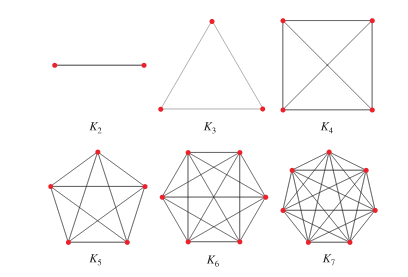
\includegraphics{images/ch2/wolfram.png}
\caption{image}
\end{figure}

A fully connected network will have a fixed number of edges as a
function of how many nodes it has. That is, for every node \(n\) a fully
connected network will have $ \frac{n(n-1)}{2} $ edges. Note that for
such networks it would be pointless to try to distinguish between nodes
using measures like centrality or community, unless the edges have
differing weights.

    It is not always possible to tell visually if a network is fully
connected , as one can see from the network below (which with 25 nodes,
remains small). In such cases machines can test the full-connectedness
of a network.

    \begin{tcolorbox}[breakable, size=fbox, boxrule=1pt, pad at break*=1mm,colback=cellbackground, colframe=cellborder]
\prompt{In}{incolor}{25}{\boxspacing}
\begin{Verbatim}[commandchars=\\\{\}]
\PY{n}{g\PYZus{}distances} \PY{o}{=} \PY{n}{load\PYZus{}graph\PYZus{}from\PYZus{}json}\PY{p}{(}\PY{l+s+s2}{\PYZdq{}}\PY{l+s+s2}{data/g\PYZus{}distances.json}\PY{l+s+s2}{\PYZdq{}}\PY{p}{)}
\PY{n}{plt}\PY{o}{.}\PY{n}{figure}\PY{p}{(}\PY{n}{figsize}\PY{o}{=}\PY{p}{(}\PY{l+m+mi}{5}\PY{p}{,}\PY{l+m+mi}{5}\PY{p}{)}\PY{p}{)}
\PY{n}{pos} \PY{o}{=} \PY{n}{nx}\PY{o}{.}\PY{n}{spring\PYZus{}layout}\PY{p}{(}\PY{n}{g\PYZus{}distances}\PY{p}{,} \PY{n}{seed}\PY{o}{=}\PY{l+m+mi}{121}\PY{p}{)}

\PY{n}{nx}\PY{o}{.}\PY{n}{draw\PYZus{}networkx\PYZus{}nodes}\PY{p}{(}\PY{n}{g\PYZus{}distances}\PY{p}{,} \PY{n}{pos}\PY{p}{)}
\PY{n}{nx}\PY{o}{.}\PY{n}{draw\PYZus{}networkx\PYZus{}edges}\PY{p}{(}\PY{n}{g\PYZus{}distances}\PY{p}{,} \PY{n}{pos}\PY{o}{=}\PY{n}{pos}\PY{p}{,} \PY{n}{edge\PYZus{}color}\PY{o}{=}\PY{l+s+s1}{\PYZsq{}}\PY{l+s+s1}{black}\PY{l+s+s1}{\PYZsq{}}\PY{p}{,} \PY{n}{alpha}\PY{o}{=}\PY{l+m+mf}{0.5}\PY{p}{)}
\end{Verbatim}
\end{tcolorbox}

            \begin{tcolorbox}[breakable, size=fbox, boxrule=.5pt, pad at break*=1mm, opacityfill=0]
\prompt{Out}{outcolor}{25}{\boxspacing}
\begin{Verbatim}[commandchars=\\\{\}]
<matplotlib.collections.LineCollection at 0x1dc695379d0>
\end{Verbatim}
\end{tcolorbox}
        
    \begin{center}
    \adjustimage{max size={0.9\linewidth}{0.9\paperheight}}{chapters/Chapter_2_Key_Concepts/output_40_1.png}
    \end{center}
    { \hspace*{\fill} \\}
    
    \begin{tcolorbox}[breakable, size=fbox, boxrule=1pt, pad at break*=1mm,colback=cellbackground, colframe=cellborder]
\prompt{In}{incolor}{26}{\boxspacing}
\begin{Verbatim}[commandchars=\\\{\}]
\PY{n}{nx}\PY{o}{.}\PY{n}{is\PYZus{}connected}\PY{p}{(}\PY{n}{g\PYZus{}distances}\PY{p}{)}
\end{Verbatim}
\end{tcolorbox}

            \begin{tcolorbox}[breakable, size=fbox, boxrule=.5pt, pad at break*=1mm, opacityfill=0]
\prompt{Out}{outcolor}{26}{\boxspacing}
\begin{Verbatim}[commandchars=\\\{\}]
True
\end{Verbatim}
\end{tcolorbox}
        
    We can also test this for our initial drone legislation example. Because
this network is a directed network, there are two ways to determine
whether the network is fully connected. A first way is by ignoring the
direction of the edges (thereby assuming an undirected network). This is
called testing whether the network is \emph{weakly} connected. As we
could see above in the network visualization, the network is fully
(weakly) connected.

    \begin{tcolorbox}[breakable, size=fbox, boxrule=1pt, pad at break*=1mm,colback=cellbackground, colframe=cellborder]
\prompt{In}{incolor}{27}{\boxspacing}
\begin{Verbatim}[commandchars=\\\{\}]
\PY{n+nb}{print}\PY{p}{(}\PY{l+s+s2}{\PYZdq{}}\PY{l+s+s2}{The network is weakly connected:}\PY{l+s+s2}{\PYZdq{}}\PY{p}{,} \PY{n}{nx}\PY{o}{.}\PY{n}{is\PYZus{}weakly\PYZus{}connected}\PY{p}{(}\PY{n}{g\PYZus{}drones1}\PY{p}{)}\PY{p}{)}
\end{Verbatim}
\end{tcolorbox}

    \begin{Verbatim}[commandchars=\\\{\}]
The network is weakly connected: True
    \end{Verbatim}

    A \emph{strongly} connected network takes the direction of the edges
into consideration. Strongly connected means there is a path between any
two nodes in both directions. Put differently, there is a path from
\(u\) to \(v\) and a path from \(v\) to \(u\) for any two nodes \(u\)
and \(v\). The drone legislation network is not strongly connected. We
could have expected this. A strongly connected network implies there are
cycles - how else could there both be a path from \(u\) to \(v\) and
from \(v\) to \(u\). Because we already concluded the drone legislation
network is a DAG, we can infer from this that it cannot be strongly
connected.

    \begin{tcolorbox}[breakable, size=fbox, boxrule=1pt, pad at break*=1mm,colback=cellbackground, colframe=cellborder]
\prompt{In}{incolor}{28}{\boxspacing}
\begin{Verbatim}[commandchars=\\\{\}]
\PY{n+nb}{print}\PY{p}{(}\PY{l+s+s2}{\PYZdq{}}\PY{l+s+s2}{The network is weakly connected:}\PY{l+s+s2}{\PYZdq{}}\PY{p}{,} \PY{n}{nx}\PY{o}{.}\PY{n}{is\PYZus{}strongly\PYZus{}connected}\PY{p}{(}\PY{n}{g\PYZus{}drones1}\PY{p}{)}\PY{p}{)}
\end{Verbatim}
\end{tcolorbox}

    \begin{Verbatim}[commandchars=\\\{\}]
The network is weakly connected: False
    \end{Verbatim}

    \hypertarget{shortest-paths}{%
\subsubsection{Shortest paths}\label{shortest-paths}}

The shortest path is the path that will reach a node in the smallest
number of steps. There can be more than one ``shortest path'' (but all
the shortest paths will have the same smallest number of steps). For
example, if we look at the kite graph, there are two shortest paths from
7 to 3, one going through 6, and another going through 5. There are
longer paths too, for example, 7 -\textgreater{} 5 -\textgreater{} 2
-\textgreater{} 3. These may not be immediately relevant, but might be
interesting possible random paths, between 7 and 3.

    \begin{tcolorbox}[breakable, size=fbox, boxrule=1pt, pad at break*=1mm,colback=cellbackground, colframe=cellborder]
\prompt{In}{incolor}{12}{\boxspacing}
\begin{Verbatim}[commandchars=\\\{\}]
\PY{n}{g\PYZus{}kite} \PY{o}{=} \PY{n}{nx}\PY{o}{.}\PY{n}{krackhardt\PYZus{}kite\PYZus{}graph}\PY{p}{(}\PY{p}{)}
\PY{n}{plt}\PY{o}{.}\PY{n}{figure}\PY{p}{(}\PY{n}{figsize}\PY{o}{=}\PY{p}{(}\PY{l+m+mi}{6}\PY{p}{,}\PY{l+m+mi}{4}\PY{p}{)}\PY{p}{)}
\PY{n}{pos} \PY{o}{=} \PY{n}{nx}\PY{o}{.}\PY{n}{spring\PYZus{}layout}\PY{p}{(}\PY{n}{g\PYZus{}kite}\PY{p}{,} \PY{n}{seed}\PY{o}{=}\PY{l+m+mi}{123}\PY{p}{)}
\PY{n}{nx}\PY{o}{.}\PY{n}{draw\PYZus{}networkx\PYZus{}nodes}\PY{p}{(}\PY{n}{g\PYZus{}kite}\PY{p}{,} \PY{n}{pos}\PY{p}{)}
\PY{n}{nx}\PY{o}{.}\PY{n}{draw\PYZus{}networkx\PYZus{}edges}\PY{p}{(}\PY{n}{g\PYZus{}kite}\PY{p}{,} \PY{n}{pos}\PY{o}{=}\PY{n}{pos}\PY{p}{)}
\PY{n}{nx}\PY{o}{.}\PY{n}{draw\PYZus{}networkx\PYZus{}edges}\PY{p}{(}\PY{n}{g\PYZus{}kite}\PY{p}{,} \PY{n}{edgelist}\PY{o}{=}\PY{p}{[}\PY{p}{(}\PY{l+m+mi}{7}\PY{p}{,}\PY{l+m+mi}{5}\PY{p}{)}\PY{p}{,}\PY{p}{(}\PY{l+m+mi}{5}\PY{p}{,}\PY{l+m+mi}{3}\PY{p}{)}\PY{p}{]}\PY{p}{,} \PY{n}{edge\PYZus{}color}\PY{o}{=}\PY{l+s+s2}{\PYZdq{}}\PY{l+s+s2}{red}\PY{l+s+s2}{\PYZdq{}}\PY{p}{,} \PY{n}{pos}\PY{o}{=}\PY{n}{pos}\PY{p}{)}
\PY{n}{nx}\PY{o}{.}\PY{n}{draw\PYZus{}networkx\PYZus{}edges}\PY{p}{(}\PY{n}{g\PYZus{}kite}\PY{p}{,} \PY{n}{edgelist}\PY{o}{=}\PY{p}{[}\PY{p}{(}\PY{l+m+mi}{7}\PY{p}{,}\PY{l+m+mi}{6}\PY{p}{)}\PY{p}{,}\PY{p}{(}\PY{l+m+mi}{6}\PY{p}{,}\PY{l+m+mi}{3}\PY{p}{)}\PY{p}{]}\PY{p}{,} \PY{n}{edge\PYZus{}color}\PY{o}{=}\PY{l+s+s2}{\PYZdq{}}\PY{l+s+s2}{green}\PY{l+s+s2}{\PYZdq{}}\PY{p}{,} \PY{n}{pos}\PY{o}{=}\PY{n}{pos}\PY{p}{)}
\PY{n}{nx}\PY{o}{.}\PY{n}{draw\PYZus{}networkx\PYZus{}labels}\PY{p}{(}\PY{n}{g\PYZus{}kite}\PY{p}{,} \PY{n}{pos}\PY{o}{=}\PY{n}{pos}\PY{p}{)}\PY{p}{;}
\end{Verbatim}
\end{tcolorbox}

    \begin{center}
    \adjustimage{max size={0.9\linewidth}{0.9\paperheight}}{chapters/Chapter_2_Key_Concepts/output_47_0.png}
    \end{center}
    { \hspace*{\fill} \\}
    
    While shortest paths can be easy to `see' in small graphs like this one,
this will not be possible in more complex graphs. Finding the shortest
path will then be a non-trivial problem. This process is automated by
network analysis libraries and programs. We use this automation to find
the shortest paths in the drone legislation network.

    \begin{tcolorbox}[breakable, size=fbox, boxrule=1pt, pad at break*=1mm,colback=cellbackground, colframe=cellborder]
\prompt{In}{incolor}{30}{\boxspacing}
\begin{Verbatim}[commandchars=\\\{\}]
\PY{c+c1}{\PYZsh{} Select source and target node}
\PY{n}{NodeA} \PY{o}{=} \PY{l+s+s1}{\PYZsq{}}\PY{l+s+s1}{2019R0945}\PY{l+s+s1}{\PYZsq{}}
\PY{n}{NodeB} \PY{o}{=} \PY{l+s+s1}{\PYZsq{}}\PY{l+s+s1}{2021R0665}\PY{l+s+s1}{\PYZsq{}}
\PY{c+c1}{\PYZsh{} For shortest path lengths between all pairs of nodes}
\PY{n}{shortest\PYZus{}paths\PYZus{}lengths} \PY{o}{=} \PY{n+nb}{dict}\PY{p}{(}\PY{n}{nx}\PY{o}{.}\PY{n}{shortest\PYZus{}path\PYZus{}length}\PY{p}{(}\PY{n}{g\PYZus{}drones1}\PY{p}{)}\PY{p}{)}
\PY{c+c1}{\PYZsh{} Print the shortest path length from one specific node to another}
\PY{n+nb}{print}\PY{p}{(}\PY{l+s+s2}{\PYZdq{}}\PY{l+s+s2}{Shortest path between}\PY{l+s+s2}{\PYZdq{}}\PY{p}{,} \PY{n}{NodeA}\PY{p}{,} \PY{l+s+s2}{\PYZdq{}}\PY{l+s+s2}{and}\PY{l+s+s2}{\PYZdq{}}\PY{p}{,} \PY{n}{NodeB}\PY{p}{,} \PY{l+s+s2}{\PYZdq{}}\PY{l+s+s2}{:}\PY{l+s+s2}{\PYZdq{}}\PY{p}{,} \PY{n}{nx}\PY{o}{.}\PY{n}{shortest\PYZus{}path\PYZus{}length}\PY{p}{(}\PY{n}{g\PYZus{}drones1}\PY{p}{,} \PY{n}{source}\PY{o}{=}\PY{n}{NodeA}\PY{p}{,} \PY{n}{target}\PY{o}{=}\PY{n}{NodeB}\PY{p}{)}\PY{p}{)}
\end{Verbatim}
\end{tcolorbox}

    \begin{Verbatim}[commandchars=\\\{\}]
Shortest path between 2019R0945 and 2021R0665 : 2
    \end{Verbatim}

    \begin{quote}
Note that because the network is directed, there is no path, and
therefore no shortest path, from 2019R0945 to 2021R0665.
\end{quote}

    Shortest paths are useful for many purposes. In the context of this
presentation, it will be seen that they are key ingredients in many
algorithms for identifying the most important or most central nodes of a
network.

For the unweighted graphs that we are using, a shortest path counts
discrete `steps' between nodes. This implies that all the nodes are a
unit distance away. However, it is also possible to have weighted paths,
as we will discuss later.

    \hypertarget{random-paths}{%
\subsubsection{Random paths}\label{random-paths}}

The length of the shortest path will be a definite number. However,
there may be a large or arbitrary number of non-shortest paths wandering
through the nodes.

A single arbitrary path will not be of much interest (why this one?, why
not another one?), but if we allow movement randomly from node to node,
these random paths - random walks - can become useful (unless the random
walk get `stuck' in a loop). We may be interested not only in the
shortest path between A and B, but in the average path distance between
A and B, taking into account routes that go more or less directly from A
to B as well as those that make longer detours. By measuring a number of
random walks for a number of nodes in the network, it will often become
clear that some nodes are more likely to be passed through than other
nodes, which suggests these nodes are more central and perhaps therefore
more relevant or interesting.

    We illustrate the shortest path with a coding example. We create a
random path with the neighbors attribute of the Graph object. The steps
are more or less like this:

\begin{enumerate}
\def\labelenumi{\arabic{enumi}.}
\tightlist
\item
  Select a number of steps for the walk. In this case four steps.
  Execute the tasks below until you hit four steps.
\item
  Select a particular node to start with, for example node 7.
\item
  Find all the neighbors of node 7 (in this case, 5, 6, 8).
\item
  Randomly choose one of these nodes to go to. Say choose node 5.
\item
  Update the value of your start position to the chosen node, in this
  case 5.
\item
  Record that you have made one step (3 to go).
\item
  If you have made less than four steps, go back to step 2. If you have
  made four steps, stop.
\end{enumerate}

These steps can be implemented in code as follows:

    \begin{tcolorbox}[breakable, size=fbox, boxrule=1pt, pad at break*=1mm,colback=cellbackground, colframe=cellborder]
\prompt{In}{incolor}{31}{\boxspacing}
\begin{Verbatim}[commandchars=\\\{\}]
\PY{c+c1}{\PYZsh{} here we are limiting the number of steps to 4, we get 5 steps in the answer because the answer includes the start node, and n is initialized at 0.}

\PY{n}{n} \PY{o}{=} \PY{l+m+mi}{0}
\PY{n}{start} \PY{o}{=} \PY{l+m+mi}{7}
\PY{n}{history} \PY{o}{=} \PY{p}{[}\PY{n}{start}\PY{p}{]}
\PY{k}{while} \PY{n}{n} \PY{o}{\PYZlt{}} \PY{l+m+mi}{4}\PY{p}{:}
  \PY{n}{my\PYZus{}neighbors} \PY{o}{=} \PY{n+nb}{list}\PY{p}{(}\PY{n}{g\PYZus{}kite}\PY{o}{.}\PY{n}{neighbors}\PY{p}{(}\PY{n}{start}\PY{p}{)}\PY{p}{)}
  \PY{n}{move\PYZus{}to\PYZus{}node} \PY{o}{=} \PY{n}{np}\PY{o}{.}\PY{n}{random}\PY{o}{.}\PY{n}{choice}\PY{p}{(}\PY{n}{my\PYZus{}neighbors}\PY{p}{)}
  \PY{n}{history}\PY{o}{.}\PY{n}{append}\PY{p}{(}\PY{n}{move\PYZus{}to\PYZus{}node}\PY{o}{.}\PY{n}{tolist}\PY{p}{(}\PY{p}{)}\PY{p}{)}
  \PY{n}{start} \PY{o}{=} \PY{n}{move\PYZus{}to\PYZus{}node}
  \PY{n}{n} \PY{o}{+}\PY{o}{=} \PY{l+m+mi}{1}

\PY{n+nb}{print}\PY{p}{(}\PY{n}{history}\PY{p}{)}
\end{Verbatim}
\end{tcolorbox}

    \begin{Verbatim}[commandchars=\\\{\}]
[7, 8, 7, 5, 7]
    \end{Verbatim}

    Most likely we will not be interest in a single random path, but in lots
of them, and they can be generated in bulk.

    \begin{tcolorbox}[breakable, size=fbox, boxrule=1pt, pad at break*=1mm,colback=cellbackground, colframe=cellborder]
\prompt{In}{incolor}{32}{\boxspacing}
\begin{Verbatim}[commandchars=\\\{\}]
\PY{n}{random\PYZus{}paths} \PY{o}{=} \PY{n}{nx}\PY{o}{.}\PY{n}{generate\PYZus{}random\PYZus{}paths}\PY{p}{(}\PY{n}{g\PYZus{}kite}\PY{p}{,} \PY{n}{sample\PYZus{}size}\PY{o}{=}\PY{l+m+mi}{10}\PY{p}{,} \PY{n}{path\PYZus{}length}\PY{o}{=}\PY{l+m+mi}{4}\PY{p}{)}
\PY{k}{for} \PY{n}{i} \PY{o+ow}{in} \PY{n}{random\PYZus{}paths}\PY{p}{:}
    \PY{n+nb}{print}\PY{p}{(}\PY{n}{i}\PY{p}{)}
\end{Verbatim}
\end{tcolorbox}

    \begin{Verbatim}[commandchars=\\\{\}]
[9, 8, 9, 8, 7]
[6, 7, 8, 9, 8]
[0, 5, 7, 6, 5]
[9, 8, 9, 8, 7]
[9, 8, 9, 8, 7]
[2, 5, 2, 0, 1]
[6, 1, 0, 1, 3]
[4, 1, 0, 5, 2]
[7, 5, 7, 5, 0]
[9, 8, 9, 8, 9]
    \end{Verbatim}

    Or, for the drone legislation example:

    \begin{tcolorbox}[breakable, size=fbox, boxrule=1pt, pad at break*=1mm,colback=cellbackground, colframe=cellborder]
\prompt{In}{incolor}{35}{\boxspacing}
\begin{Verbatim}[commandchars=\\\{\}]
\PY{c+c1}{\PYZsh{} Get the list of all nodes in the graph}
\PY{n}{nodes} \PY{o}{=} \PY{n+nb}{list}\PY{p}{(}\PY{n}{g\PYZus{}drones1}\PY{o}{.}\PY{n}{nodes}\PY{p}{(}\PY{p}{)}\PY{p}{)}  \PY{c+c1}{\PYZsh{} Ensure you use .nodes() to get the nodes from the graph}

\PY{c+c1}{\PYZsh{} Generate 10 random paths}
\PY{n}{random\PYZus{}paths} \PY{o}{=} \PY{p}{[}\PY{p}{]}
\PY{k}{for} \PY{n}{\PYZus{}} \PY{o+ow}{in} \PY{n+nb}{range}\PY{p}{(}\PY{l+m+mi}{10}\PY{p}{)}\PY{p}{:}
    \PY{c+c1}{\PYZsh{} Randomly select source and target nodes}
    \PY{n}{source}\PY{p}{,} \PY{n}{target} \PY{o}{=} \PY{n}{random}\PY{o}{.}\PY{n}{sample}\PY{p}{(}\PY{n}{nodes}\PY{p}{,} \PY{l+m+mi}{2}\PY{p}{)}  \PY{c+c1}{\PYZsh{} Ensure source and target are different}

    \PY{k}{try}\PY{p}{:}
        \PY{c+c1}{\PYZsh{} Find the shortest path between the random nodes}
        \PY{n}{path} \PY{o}{=} \PY{n}{nx}\PY{o}{.}\PY{n}{shortest\PYZus{}path}\PY{p}{(}\PY{n}{g\PYZus{}drones1}\PY{p}{,} \PY{n}{source}\PY{o}{=}\PY{n}{source}\PY{p}{,} \PY{n}{target}\PY{o}{=}\PY{n}{target}\PY{p}{)}
        \PY{n}{random\PYZus{}paths}\PY{o}{.}\PY{n}{append}\PY{p}{(}\PY{n}{path}\PY{p}{)}
    \PY{k}{except} \PY{n}{nx}\PY{o}{.}\PY{n}{NetworkXNoPath}\PY{p}{:}
        \PY{c+c1}{\PYZsh{} If no path exists between the selected nodes, skip or handle it as needed}
        \PY{n+nb}{print}\PY{p}{(}\PY{l+s+sa}{f}\PY{l+s+s2}{\PYZdq{}}\PY{l+s+s2}{No path between }\PY{l+s+si}{\PYZob{}}\PY{n}{source}\PY{l+s+si}{\PYZcb{}}\PY{l+s+s2}{ and }\PY{l+s+si}{\PYZob{}}\PY{n}{target}\PY{l+s+si}{\PYZcb{}}\PY{l+s+s2}{\PYZdq{}}\PY{p}{)}
        \PY{k}{continue}

\PY{c+c1}{\PYZsh{} Print the random paths}
\PY{k}{for} \PY{n}{i}\PY{p}{,} \PY{n}{path} \PY{o+ow}{in} \PY{n+nb}{enumerate}\PY{p}{(}\PY{n}{random\PYZus{}paths}\PY{p}{)}\PY{p}{:}
    \PY{n+nb}{print}\PY{p}{(}\PY{l+s+sa}{f}\PY{l+s+s2}{\PYZdq{}}\PY{l+s+s2}{Random Path }\PY{l+s+si}{\PYZob{}}\PY{n}{i}\PY{o}{+}\PY{l+m+mi}{1}\PY{l+s+si}{\PYZcb{}}\PY{l+s+s2}{: }\PY{l+s+si}{\PYZob{}}\PY{n}{path}\PY{l+s+si}{\PYZcb{}}\PY{l+s+s2}{\PYZdq{}}\PY{p}{)}
\end{Verbatim}
\end{tcolorbox}

    \begin{Verbatim}[commandchars=\\\{\}]
No path between 2019R0947 and 2014R1321
No path between 2020R0639 and 2014R0376
No path between 2021R0665 and 2014R1321
No path between 2019R0947 and 2000L0031
No path between 2004R0551 and 2014L0030
No path between 2001L0095 and 2004R0551
No path between 2020R0746 and 2014R1321
No path between 2006L0042 and 2023D0746
No path between 2009L0048 and 2014L0030
Random Path 1: ['2019R0945', '2000L0031']
    \end{Verbatim}

    \hypertarget{weighted-edges}{%
\subsubsection{Weighted edges}\label{weighted-edges}}

An edge can show that there is a relationship between nodes A and B. The
nature of that relationship can be many things, such as there being a
train between A and B, or that case A cites case B. In these instances
the relationship is binary: There either is a connection or there is
not.

However, there is a range of cases where one wants to record the
strength of a connection and not just its presence. For example, one
might want to record not only that there is train path from A to B but
also how long that path is in terms of kilometers. We might want to
score not only that case A cites case B but also how many times case B
is cited by case A. We can add this attribute to the edge by giving
weights to edges. For instance, if case A cites case B four times, the
edge weight becomes four.

Weighted networks can be represented visually in an intuitive way by
using different colors or line styles for their edges. Below is a
network using a document similarity matrix. This matrix records how
close two documents are in light of the tokens they share (Jaccard
distance) and scores them with 1 if they are identical, and 0 if they
are completely different. It is made of a set of ECHR Grand Chamber
judgments on the extraterritorial application of fundamental rights.

    In the process of comparing the distance between each document, this
dataframe is turned into a matrix, and that can be used to build a
network. Please see Appendix 1: ``Text Similarity Networks'' for more
details of how this can be done.

The purpose of this example is to show that if you graph the network
without consideration of weight, it gives you a fully connected network,
which is a nice geometrical figure, but not very informative. Every
document was compared to every other document, so every node is on step
(one degree) of separation from every other and so every node has the
exact same number of neighbors.

A more informative network structure can be shown if we take
consideration of weight. One way to do this is to pick only the edges
whose weight meets a certain test. Here we are simply whose weight
surpases the mean weight plus one standard deviation.

    \begin{tcolorbox}[breakable, size=fbox, boxrule=1pt, pad at break*=1mm,colback=cellbackground, colframe=cellborder]
\prompt{In}{incolor}{36}{\boxspacing}
\begin{Verbatim}[commandchars=\\\{\}]
\PY{n}{g\PYZus{}distances} \PY{o}{=} \PY{n}{load\PYZus{}graph\PYZus{}from\PYZus{}json}\PY{p}{(}\PY{l+s+s2}{\PYZdq{}}\PY{l+s+s2}{data/g\PYZus{}distances.json}\PY{l+s+s2}{\PYZdq{}}\PY{p}{)}
\PY{n}{mean\PYZus{}simil} \PY{o}{=} \PY{n}{np}\PY{o}{.}\PY{n}{mean}\PY{p}{(}\PY{p}{[}\PY{n}{z} \PY{k}{for} \PY{n}{x}\PY{p}{,}\PY{n}{y}\PY{p}{,}\PY{n}{z} \PY{o+ow}{in} \PY{n}{g\PYZus{}distances}\PY{o}{.}\PY{n}{edges}\PY{o}{.}\PY{n}{data}\PY{p}{(}\PY{l+s+s2}{\PYZdq{}}\PY{l+s+s2}{weight}\PY{l+s+s2}{\PYZdq{}}\PY{p}{)}\PY{p}{]}\PY{p}{)}
\PY{n}{std\PYZus{}mimil} \PY{o}{=} \PY{n}{np}\PY{o}{.}\PY{n}{std}\PY{p}{(}\PY{p}{[}\PY{n}{z} \PY{k}{for} \PY{n}{x}\PY{p}{,}\PY{n}{y}\PY{p}{,}\PY{n}{z} \PY{o+ow}{in} \PY{n}{g\PYZus{}distances}\PY{o}{.}\PY{n}{edges}\PY{o}{.}\PY{n}{data}\PY{p}{(}\PY{l+s+s2}{\PYZdq{}}\PY{l+s+s2}{weight}\PY{l+s+s2}{\PYZdq{}}\PY{p}{)}\PY{p}{]}\PY{p}{)}

\PY{n}{fig}\PY{p}{,} \PY{n}{ax} \PY{o}{=} \PY{n}{plt}\PY{o}{.}\PY{n}{subplots}\PY{p}{(}\PY{n}{nrows}\PY{o}{=}\PY{l+m+mi}{1}\PY{p}{,} \PY{n}{ncols}\PY{o}{=}\PY{l+m+mi}{2}\PY{p}{,}\PY{n}{figsize}\PY{o}{=}\PY{p}{(}\PY{l+m+mi}{16}\PY{p}{,}\PY{l+m+mi}{8}\PY{p}{)}\PY{p}{)}
\PY{n}{pos} \PY{o}{=} \PY{n}{nx}\PY{o}{.}\PY{n}{spring\PYZus{}layout}\PY{p}{(}\PY{n}{g\PYZus{}distances}\PY{p}{,} \PY{n}{seed}\PY{o}{=}\PY{l+m+mi}{121}\PY{p}{)}


\PY{n}{nx}\PY{o}{.}\PY{n}{draw\PYZus{}networkx\PYZus{}nodes}\PY{p}{(}\PY{n}{g\PYZus{}distances}\PY{p}{,} \PY{n}{pos}\PY{p}{,} \PY{n}{ax}\PY{o}{=}\PY{n}{ax}\PY{p}{[}\PY{l+m+mi}{0}\PY{p}{]}\PY{p}{)}
\PY{n}{nx}\PY{o}{.}\PY{n}{draw\PYZus{}networkx\PYZus{}edges}\PY{p}{(}\PY{n}{g\PYZus{}distances}\PY{p}{,} \PY{n}{pos}\PY{o}{=}\PY{n}{pos}\PY{p}{,} \PY{n}{edge\PYZus{}color}\PY{o}{=}\PY{l+s+s1}{\PYZsq{}}\PY{l+s+s1}{green}\PY{l+s+s1}{\PYZsq{}}\PY{p}{,} \PY{n}{ax}\PY{o}{=}\PY{n}{ax}\PY{p}{[}\PY{l+m+mi}{0}\PY{p}{]}\PY{p}{,} \PY{n}{alpha}\PY{o}{=}\PY{l+m+mf}{0.5}\PY{p}{)}
\PY{n}{nx}\PY{o}{.}\PY{n}{draw\PYZus{}networkx\PYZus{}labels}\PY{p}{(}\PY{n}{g\PYZus{}distances}\PY{p}{,} \PY{n}{pos}\PY{o}{=}\PY{n}{pos}\PY{p}{,} \PY{n}{font\PYZus{}size}\PY{o}{=}\PY{l+m+mi}{7}\PY{p}{,} \PY{n}{ax} \PY{o}{=} \PY{n}{ax}\PY{p}{[}\PY{l+m+mi}{0}\PY{p}{]}\PY{p}{)}\PY{p}{;}

\PY{n}{nx}\PY{o}{.}\PY{n}{draw\PYZus{}networkx\PYZus{}nodes}\PY{p}{(}\PY{n}{g\PYZus{}distances}\PY{p}{,} \PY{n}{pos}\PY{p}{,} \PY{n}{ax}\PY{o}{=}\PY{n}{ax}\PY{p}{[}\PY{l+m+mi}{1}\PY{p}{]}\PY{p}{)}
\PY{n}{lowweight} \PY{o}{=} \PY{p}{[}\PY{n}{e} \PY{k}{for} \PY{n}{e} \PY{o+ow}{in} \PY{n}{g\PYZus{}distances}\PY{o}{.}\PY{n}{edges} \PY{k}{if} \PY{n}{g\PYZus{}distances}\PY{o}{.}\PY{n}{edges}\PY{p}{[}\PY{n}{e}\PY{p}{]}\PY{p}{[}\PY{l+s+s1}{\PYZsq{}}\PY{l+s+s1}{weight}\PY{l+s+s1}{\PYZsq{}}\PY{p}{]} \PY{o}{\PYZlt{}} \PY{n}{mean\PYZus{}simil}\PY{o}{+}\PY{n}{std\PYZus{}mimil}\PY{p}{]}
\PY{n}{highweight} \PY{o}{=} \PY{p}{[}\PY{n}{e} \PY{k}{for} \PY{n}{e} \PY{o+ow}{in} \PY{n}{g\PYZus{}distances}\PY{o}{.}\PY{n}{edges} \PY{k}{if} \PY{n}{g\PYZus{}distances}\PY{o}{.}\PY{n}{edges}\PY{p}{[}\PY{n}{e}\PY{p}{]}\PY{p}{[}\PY{l+s+s1}{\PYZsq{}}\PY{l+s+s1}{weight}\PY{l+s+s1}{\PYZsq{}}\PY{p}{]} \PY{o}{\PYZgt{}} \PY{n}{mean\PYZus{}simil}\PY{o}{+}\PY{n}{std\PYZus{}mimil}\PY{p}{]}
\PY{n}{nx}\PY{o}{.}\PY{n}{draw\PYZus{}networkx\PYZus{}edges}\PY{p}{(}\PY{n}{g\PYZus{}distances}\PY{p}{,} \PY{n}{edgelist}\PY{o}{=}\PY{n}{highweight}\PY{p}{,} \PY{n}{pos}\PY{o}{=}\PY{n}{pos}\PY{p}{,} \PY{n}{edge\PYZus{}color}\PY{o}{=}\PY{l+s+s1}{\PYZsq{}}\PY{l+s+s1}{green}\PY{l+s+s1}{\PYZsq{}}\PY{p}{,} \PY{n}{ax}\PY{o}{=}\PY{n}{ax}\PY{p}{[}\PY{l+m+mi}{1}\PY{p}{]}\PY{p}{)}
\PY{n}{nx}\PY{o}{.}\PY{n}{draw\PYZus{}networkx\PYZus{}labels}\PY{p}{(}\PY{n}{g\PYZus{}distances}\PY{p}{,} \PY{n}{pos}\PY{o}{=}\PY{n}{pos}\PY{p}{,} \PY{n}{font\PYZus{}size}\PY{o}{=}\PY{l+m+mi}{7}\PY{p}{,} \PY{n}{ax} \PY{o}{=} \PY{n}{ax}\PY{p}{[}\PY{l+m+mi}{1}\PY{p}{]}\PY{p}{)}\PY{p}{;}
\end{Verbatim}
\end{tcolorbox}

    \begin{center}
    \adjustimage{max size={0.9\linewidth}{0.9\paperheight}}{chapters/Chapter_2_Key_Concepts/output_61_0.png}
    \end{center}
    { \hspace*{\fill} \\}
    
    We stated that assessing centrality or community of fully connected
networks can be pointless, for all the nodes are then by definition
connected to all the other nodes, and so they will get identical scores.
However, in weighted networks it is not pointless to assess the
centrality or community of its nodes, because the edges have different
weights. This is illustrated in the section on closeness centrality
below.

Calculating shortest paths is different for weighted edges than for
unweighted edges. In unweighted graphs it would be a matter of counting
the steps on different paths and finding the one with the lowest number
of steps, whereas in weighted graphs the procedure is to count the steps
and multiply every step by its weight.

Also note that the weight can represent closeness or distance. If it
represents distance, then one must simply multiply by it. If it
represents closeness, we need to convert it into distance by using its
reciprocal.

\[ distance = \frac{1}{closeness} \]

    \hypertarget{network-density}{%
\subsubsection{Network Density}\label{network-density}}

Recall the fully connected networks discussed earlier:

\begin{figure}
\centering
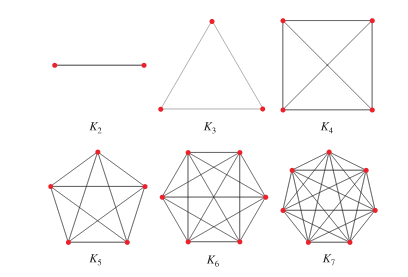
\includegraphics{images/ch2/wolfram.png}
\caption{image}
\end{figure}

    Since every node here will be connected to every other node (there are
no strangers, everyone is a neighbor of everyone else, everyone has
maximum popularity) it can be said that these networks are maximally
dense.

A maximally dense network will have $ \frac{n(n-1)}{2} $ edges.
Consequently, a network with 3 nodes can have a maximum of 3 edges, a
network with 4 nodes 6 edges, a network with 5 nodes 10 edges, and so
forth.

The network density will be the ratio of the number of edges actually
present \$ m \$ to the hypothetical maximum, in other words:

\[ \frac{m}{n(n-1)/2} \]

    Using this formula, we can calculate the density of our drone
legislation network. The density is fairly low (.10), which coincides
with a visual inspection of the network, where we can observe that nodes
are frequently connected to one other node but not to other nodes.
Consequently, the number of actual edges to a node is far less than the
number of possible edges to other nodes.

    \begin{tcolorbox}[breakable, size=fbox, boxrule=1pt, pad at break*=1mm,colback=cellbackground, colframe=cellborder]
\prompt{In}{incolor}{37}{\boxspacing}
\begin{Verbatim}[commandchars=\\\{\}]
\PY{n}{n} \PY{o}{=} \PY{n}{g\PYZus{}drones1}\PY{o}{.}\PY{n}{number\PYZus{}of\PYZus{}nodes}\PY{p}{(}\PY{p}{)}
\PY{n}{m} \PY{o}{=} \PY{n}{g\PYZus{}drones1}\PY{o}{.}\PY{n}{number\PYZus{}of\PYZus{}edges}\PY{p}{(}\PY{p}{)}

\PY{k}{if} \PY{n}{n} \PY{o}{\PYZgt{}} \PY{l+m+mi}{1}\PY{p}{:}
    \PY{n}{density} \PY{o}{=} \PY{n}{m} \PY{o}{/} \PY{p}{(}\PY{n}{n} \PY{o}{*} \PY{p}{(}\PY{n}{n} \PY{o}{\PYZhy{}} \PY{l+m+mi}{1}\PY{p}{)} \PY{o}{/} \PY{l+m+mi}{2}\PY{p}{)}
\PY{k}{else}\PY{p}{:}
    \PY{n}{density} \PY{o}{=} \PY{l+m+mi}{0}  \PY{c+c1}{\PYZsh{} The density of a graph with 1 or 0 nodes is defined as 0}

\PY{n+nb}{print}\PY{p}{(}\PY{l+s+s2}{\PYZdq{}}\PY{l+s+s2}{Density of the graph:}\PY{l+s+s2}{\PYZdq{}}\PY{p}{,} \PY{n}{density}\PY{p}{)}
\end{Verbatim}
\end{tcolorbox}

    \begin{Verbatim}[commandchars=\\\{\}]
Density of the graph: 0.09881422924901186
    \end{Verbatim}

    \hypertarget{eccentricity-and-network-diameter}{%
\subsubsection{Eccentricity and Network
Diameter}\label{eccentricity-and-network-diameter}}

Next we need to consider eccentricity. Eccentricity records the longest
shortest path between every node. In the kite graph above, we can see
that the eccentricity of node 9 is 4, as the maximum shortest path that
exist between that node and some other node is four steps. Node 7, by
contrast, has a maximum eccentricity of 2, as the longest shortest path
that exist between it any other node is just 2.

Just as we can be interested in what is the center of a network, we can
be interested in how large the network is. However, one cannot just
`eye' a network graph to get a sense of its dimensions, because a graph
can be plotted in many different ways and still be the same network.

The diameter of a network is very simple to calculate. It is just the
maximum eccentricity value. A network is as wide as the longest shortest
path that it includes. For the kite network, no node is further away
than four steps from any other (that is the longest shortest path) and
thus that is its diameter.

    \begin{tcolorbox}[breakable, size=fbox, boxrule=1pt, pad at break*=1mm,colback=cellbackground, colframe=cellborder]
\prompt{In}{incolor}{38}{\boxspacing}
\begin{Verbatim}[commandchars=\\\{\}]
\PY{n+nb}{print}\PY{p}{(}\PY{l+s+s2}{\PYZdq{}}\PY{l+s+s2}{Diameter of the connected graph:}\PY{l+s+s2}{\PYZdq{}}\PY{p}{,} \PY{n}{nx}\PY{o}{.}\PY{n}{diameter}\PY{p}{(}\PY{n}{g\PYZus{}kite}\PY{p}{)}\PY{p}{)}
\end{Verbatim}
\end{tcolorbox}

    \begin{Verbatim}[commandchars=\\\{\}]
Diameter of the connected graph: 4
    \end{Verbatim}

    We can also perform the calculation for the drone legislation network.
Because this network is a directed network, we will first convert it to
an undirected network, which makes the interpretation more
straightforward.

    \begin{tcolorbox}[breakable, size=fbox, boxrule=1pt, pad at break*=1mm,colback=cellbackground, colframe=cellborder]
\prompt{In}{incolor}{39}{\boxspacing}
\begin{Verbatim}[commandchars=\\\{\}]
\PY{c+c1}{\PYZsh{} Create a weakly connected version of the graph}
\PY{n}{g\PYZus{}weak} \PY{o}{=} \PY{n}{g\PYZus{}drones1}\PY{o}{.}\PY{n}{to\PYZus{}undirected}\PY{p}{(}\PY{p}{)}
\PY{c+c1}{\PYZsh{} Calculate the diamater}
\PY{n+nb}{print}\PY{p}{(}\PY{l+s+s2}{\PYZdq{}}\PY{l+s+s2}{Diameter of the weakly connected graph:}\PY{l+s+s2}{\PYZdq{}}\PY{p}{,} \PY{n}{nx}\PY{o}{.}\PY{n}{diameter}\PY{p}{(}\PY{n}{g\PYZus{}weak}\PY{p}{)}\PY{p}{)}
\end{Verbatim}
\end{tcolorbox}

    \begin{Verbatim}[commandchars=\\\{\}]
Diameter of the weakly connected graph: 3
    \end{Verbatim}

    \hypertarget{ego-networks}{%
\subsection{2.12 Ego Networks}\label{ego-networks}}

One important type of subgraph is the ego network, which is centered on
one particular node (the `ego' or self) and then contains only those
nodes that have a path to the ego within a given radius. That is to say,
we can see only the nodes that are a defined number of steps away from
the ego.

The drone legislation example is an ego network. This is the result of
the way in which it was construed. By including all references in the a
specific node (node 2019R0945), the references to the node, and the
references to the references to the node, the resulting network is one
that is centered around the source node (node 2019R0945).

    An ego network can be useful to zoom in on one particular set of
relations. For example, using the karate club graph we can use ego
networks to see all the nodes that are one step away from the karate
instructor (node 33 in the networkx version of the dataset).

    \begin{tcolorbox}[breakable, size=fbox, boxrule=1pt, pad at break*=1mm,colback=cellbackground, colframe=cellborder]
\prompt{In}{incolor}{40}{\boxspacing}
\begin{Verbatim}[commandchars=\\\{\}]
\PY{n}{fig}\PY{p}{,} \PY{n}{ax} \PY{o}{=} \PY{n}{plt}\PY{o}{.}\PY{n}{subplots}\PY{p}{(}\PY{n}{nrows}\PY{o}{=}\PY{l+m+mi}{1}\PY{p}{,} \PY{n}{ncols}\PY{o}{=}\PY{l+m+mi}{2}\PY{p}{,} \PY{n}{figsize}\PY{o}{=}\PY{p}{(}\PY{l+m+mi}{10}\PY{p}{,}\PY{l+m+mi}{6}\PY{p}{)}\PY{p}{)}
\PY{n}{g\PYZus{}karate} \PY{o}{=} \PY{n}{nx}\PY{o}{.}\PY{n}{karate\PYZus{}club\PYZus{}graph}\PY{p}{(}\PY{p}{)}
\PY{n}{ego\PYZus{}karate} \PY{o}{=} \PY{n}{nx}\PY{o}{.}\PY{n}{ego\PYZus{}graph}\PY{p}{(}\PY{n}{g\PYZus{}karate}\PY{p}{,} \PY{l+m+mi}{33}\PY{p}{)}
\PY{n}{pos} \PY{o}{=} \PY{n}{nx}\PY{o}{.}\PY{n}{spring\PYZus{}layout}\PY{p}{(}\PY{n}{g\PYZus{}karate}\PY{p}{,} \PY{n}{seed}\PY{o}{=}\PY{l+m+mi}{123}\PY{p}{)}
\PY{n}{nx}\PY{o}{.}\PY{n}{draw\PYZus{}networkx\PYZus{}nodes}\PY{p}{(}\PY{n}{ego\PYZus{}karate}\PY{p}{,} \PY{n}{pos}\PY{o}{=}\PY{n}{pos}\PY{p}{,} \PY{n}{ax}\PY{o}{=}\PY{n}{ax}\PY{p}{[}\PY{l+m+mi}{0}\PY{p}{]}\PY{p}{,} \PY{n}{node\PYZus{}color}\PY{o}{=}\PY{l+s+s2}{\PYZdq{}}\PY{l+s+s2}{tab:red}\PY{l+s+s2}{\PYZdq{}}\PY{p}{)}
\PY{n}{nx}\PY{o}{.}\PY{n}{draw\PYZus{}networkx\PYZus{}labels}\PY{p}{(}\PY{n}{ego\PYZus{}karate}\PY{p}{,} \PY{n}{pos}\PY{o}{=}\PY{n}{pos}\PY{p}{,} \PY{n}{ax}\PY{o}{=}\PY{n}{ax}\PY{p}{[}\PY{l+m+mi}{0}\PY{p}{]}\PY{p}{)}
\PY{n}{nx}\PY{o}{.}\PY{n}{draw\PYZus{}networkx\PYZus{}edges}\PY{p}{(}\PY{n}{ego\PYZus{}karate}\PY{p}{,} \PY{n}{pos}\PY{o}{=}\PY{n}{pos}\PY{p}{,} \PY{n}{ax}\PY{o}{=}\PY{n}{ax}\PY{p}{[}\PY{l+m+mi}{0}\PY{p}{]}\PY{p}{)}
\PY{n}{nx}\PY{o}{.}\PY{n}{draw\PYZus{}networkx\PYZus{}nodes}\PY{p}{(}\PY{n}{g\PYZus{}karate}\PY{p}{,} \PY{n}{pos}\PY{o}{=}\PY{n}{pos}\PY{p}{,} \PY{n}{ax}\PY{o}{=}\PY{n}{ax}\PY{p}{[}\PY{l+m+mi}{1}\PY{p}{]}\PY{p}{)}
\PY{n}{nx}\PY{o}{.}\PY{n}{draw\PYZus{}networkx\PYZus{}nodes}\PY{p}{(}\PY{n}{ego\PYZus{}karate}\PY{p}{,} \PY{n}{pos}\PY{o}{=}\PY{n}{pos}\PY{p}{,} \PY{n}{node\PYZus{}color}\PY{o}{=}\PY{l+s+s2}{\PYZdq{}}\PY{l+s+s2}{tab:red}\PY{l+s+s2}{\PYZdq{}}\PY{p}{,} \PY{n}{ax}\PY{o}{=}\PY{n}{ax}\PY{p}{[}\PY{l+m+mi}{1}\PY{p}{]}\PY{p}{)}
\PY{n}{nx}\PY{o}{.}\PY{n}{draw\PYZus{}networkx\PYZus{}labels}\PY{p}{(}\PY{n}{g\PYZus{}karate}\PY{p}{,} \PY{n}{pos}\PY{o}{=}\PY{n}{pos}\PY{p}{,} \PY{n}{ax}\PY{o}{=}\PY{n}{ax}\PY{p}{[}\PY{l+m+mi}{1}\PY{p}{]}\PY{p}{)}
\PY{n}{nx}\PY{o}{.}\PY{n}{draw\PYZus{}networkx\PYZus{}edges}\PY{p}{(}\PY{n}{g\PYZus{}karate}\PY{p}{,} \PY{n}{pos}\PY{o}{=}\PY{n}{pos}\PY{p}{,} \PY{n}{ax}\PY{o}{=}\PY{n}{ax}\PY{p}{[}\PY{l+m+mi}{1}\PY{p}{]}\PY{p}{)}
\PY{n}{ax}\PY{p}{[}\PY{l+m+mi}{0}\PY{p}{]}\PY{o}{.}\PY{n}{set\PYZus{}title}\PY{p}{(}\PY{l+s+s2}{\PYZdq{}}\PY{l+s+s2}{Ego network of the Karate instructor}\PY{l+s+s2}{\PYZdq{}}\PY{p}{)}
\PY{n}{ax}\PY{p}{[}\PY{l+m+mi}{1}\PY{p}{]}\PY{o}{.}\PY{n}{set\PYZus{}title}\PY{p}{(}\PY{l+s+s2}{\PYZdq{}}\PY{l+s+s2}{Superimposed on the whole network}\PY{l+s+s2}{\PYZdq{}}\PY{p}{)}\PY{p}{;}
\end{Verbatim}
\end{tcolorbox}

    \begin{center}
    \adjustimage{max size={0.9\linewidth}{0.9\paperheight}}{chapters/Chapter_2_Key_Concepts/output_73_0.png}
    \end{center}
    { \hspace*{\fill} \\}
    

    % Add a bibliography block to the postdoc
    
    
    

